\documentclass[10pt]{report}
\usepackage{blindtext}
\usepackage{times}
\usepackage{graphicx}
\usepackage{geometry}
\usepackage{sectsty}
\usepackage{float}
\usepackage{array}
% \usepackage[backend=biber,bibencoding=latin1]{biblatex}
\chapterfont{\centering}
\usepackage{enumitem}
\usepackage{enumerate}
\usepackage{listings}
\usepackage{color}
\usepackage{ragged2e}
\usepackage{pdfpages} 
\usepackage{draftwatermark}
\SetWatermarkText{} % Keep clean watermark or blank

\usepackage[headheight=0pt,headsep=0pt]{geometry}

\usepackage{xcolor}
\definecolor{mybrown}{RGB}{131, 96, 65}
\definecolor{gray}{rgb}{0.5,0.5,0.5}
\definecolor{mauve}{rgb}{0.58,0,0.82}

\makeatletter
\def\@makechapterhead#1{%
  {\parindent \z@ \centering\normalfont
    \ifnum \c@secnumdepth >\m@ne
        \huge\bfseries \@chapapp\space \thechapter
        \par\nobreak
        \vskip 20\p@
    \fi
    \interlinepenalty\@M
    \Huge \bfseries #1\par\nobreak
    \vskip 40\p@
  }}
\def\@makeschapterhead#1{%
  {\parindent \z@ \centering
    \normalfont
    \interlinepenalty\@M
    \Huge \bfseries  #1\par\nobreak
    \vskip 40\p@
  }}
\makeatother

\lstset{ %
 language=Python,
 basicstyle=\footnotesize\ttfamily,
 numbers=left,
 numberstyle=\tiny\color{gray},
 stepnumber=1,
 numbersep=5pt,
 backgroundcolor=\color{white},
 showspaces=false,
 showstringspaces=false,
 showtabs=false,
 frame=single,
 rulecolor=\color{black},
 tabsize=2,
 captionpos=b,
 breaklines=true,
 breakatwhitespace=false,
 title=\lstname,
 keywordstyle=\color{blue},
 commentstyle=\color{gray},
 stringstyle=\color{mauve},
 escapeinside={\%*}{*)},
 morekeywords={*,self}
}

\geometry{a4paper,total={180mm,250mm},left=20mm,top=20mm, right=20mm}

\begin{document}

% -------------------------------------------------------------
% Title Page 1 (Color: mybrown)
% -------------------------------------------------------------
\pagecolor{mybrown}
\color{white}

\newpage
\begin{center}
\hspace{10cm}
\LARGE{\textsc {\textbf{\textcolor{white}{Batch No:MI1207}}}}\\[0.2cm]

\thispagestyle{empty}
\LARGE{\textsc {\textbf{\textcolor{white}{AI-Based Smart Classroom Monitoring System}}}}\\[0.2cm]

\vspace{0.2cm}
\Large{\textit{\textcolor{white}{Minor Project-I  report submitted in partial fulfillment of the requirement for award of the degree of}}}\\[0.3cm]

\Large{\textbf{\textcolor{white}{Bachelor of Technology in Computer Science \& Engineering}}}

\vspace{0.5cm}
\Large{\textbf{\textcolor{white}{By}}}\\[0.5cm]

\begin{table}[h]
\centering
\Large{\textcolor{white}{
\begin{tabular}{>{\bfseries}lc>{\bfseries}r}
BINGINAPALLI SUMANTH & (24UECS0446) & (VTU29602)\\
BOLLINENI NAGA KOUSHIK & (24UECS0458) & (VTU29411)\\
CHITTEMREDDY HEMANTH KUMAR & (24UECS0500) & (VTU29443)\\
\end{tabular}}}
\end{table}

\vspace{0.5cm}
\large{\textit{\textcolor{white}{Under the guidance of}}}\\
\large{\textit{\textcolor{white}{Dr. Sumithra M, M.E., Ph.D., \\Assistant Professor (Senior Grade)}}}\\

\vspace{0.5cm}
\includegraphics[scale=0.5]{images/Vel tech-Logo.png}\\

\vspace{1cm}
\large{\textbf{\textcolor{white}{DEPARTMENT OF COMPUTER SCIENCE AND ENGINEERING}}}\\
\large{\textbf{\textcolor{white}{SCHOOL OF COMPUTING}}}\\

\vspace{0.5cm}
\Large{\textbf{\textcolor{white}{VEL TECH RANGARAJAN DR. SAGUNTHALA R\&D INSTITUTE OF SCIENCE AND TECHNOLOGY}}}\\

\Large{\textbf{\textcolor{white}{(Deemed to be University)}}}\\
\Large{\textbf{\textcolor{white}{Accredited by NAAC with A++ Grade}}}\\
\large{\textbf{\textcolor{white}{CHENNAI 600 062, TAMILNADU, INDIA}}}

\vspace{0.4cm}
\large{\textbf{\textcolor{white}{NOV 2026}}}

\end{center}

\newpage
\nopagecolor
\color{black}

% -------------------------------------------------------------
% Title Page 2 (White with Blue text)
% -------------------------------------------------------------
\newpage
\begin{center}
\hspace{10cm}
\LARGE{\textsc {\textbf{\textcolor{blue}{Batch No:MI1207}}}}\\[0.2cm]
\thispagestyle{empty}
\LARGE{\textsc {\textbf{\textcolor{blue}{AI-Based Smart Classroom Monitoring System}}}}\\[0.2cm]
\vspace{0.2cm}
\Large{\textit{\textcolor{blue}{\\Minor Project-I  report submitted \\in partial fulfillment of the
requirement
for award of the degree of}}}\\[0.3cm]
\Large{\textbf{\textcolor{blue}{\\Bachelor of Technology\\in \\Computer Science \& Engineering}}}
\vspace{0.5cm}
\Large{\textbf{\textcolor{blue}{\\By}}}\\[0.5cm]
\begin{table}[h]
\centering
\Large{\textcolor{blue}{
\begin{tabular}{>{\bfseries}lc>{\bfseries}r}
BINGINAPALLI SUMANTH & (24UECS0446) & (VTU29602)\\
BOLLINENI NAGA KOUSHIK & (24UECS0458) & (VTU29411)\\
CHITTEMREDDY HEMANTH KUMAR & (24UECS0500) & (VTU29443)\\
\end{tabular}}}
\end{table}
\vspace{0.5cm}
\large{\textit{\textcolor{blue}{Under the guidance of}}}\\
\large{\textit{\textcolor{blue}{Dr. Sumithra M, M.E., Ph.D.,\\
Assistant Professor (Senior Grade)}
}}\\
\vspace{0.5cm}
\includegraphics[scale=0.5]{images/Vel tech-Logo.png}\\
\vspace{1cm}
\large{\textbf{\textcolor{blue}{DEPARTMENT OF COMPUTER SCIENCE AND ENGINEERING}}}\\

\large{\textbf{\textcolor{blue}{SCHOOL OF COMPUTING}}}\\
\vspace{0.5cm}
\Large{\textbf{\textcolor{blue}{VEL TECH RANGARAJAN DR. SAGUNTHALA R\&D INSTITUTE OF
SCIENCE AND TECHNOLOGY\\
\vspace{0.2cm}
(Deemed to be University Estd u/s 3 of UGC Act,
1956)}}}\\\Large{\textbf{\textcolor{blue}{Accredited by NAAC with A++ Grade}}}\\
\large{\textbf{\textcolor{blue}{CHENNAI 600 062, TAMILNADU, INDIA}}}
\vspace{0.4cm}
\large{\textbf{\textcolor{blue}{\\NOV 2026}}}\\
\end{center}

% -------------------------------------------------------------
% CERTIFICATE
% -------------------------------------------------------------
\newgeometry{left=20mm,top=20mm, right=20mm} 
\begin{center}
{\Huge \textbf{CERTIFICATE}}\\[1cm]
\end{center}
\linespread{1.5}
\large{It is certified that the work contained in the project report titled \textbf{"AI-BASED SMART CLASSROOM MONITORING SYSTEM"} by \textbf{"BINGINAPALLI SUMANTH (24UECS0446), BOLLINENI NAGA KOUSHIK (24UECS0458), CHITTEMREDDY HEMANTH KUMAR (24UECS0500)"} has been carried out under my supervision and that this work has not
been submitted elsewhere for a degree.}
\vspace{1.5cm}
\begin{flushright}
\textbf{Signature of Supervisor\\Dr. Sumithra M, M.E., Ph.D.\\Assistant Professor (Senior Grade)\\Computer Science \&
Engineering\\School of Computing\\Vel Tech Rangarajan Dr. Sagunthala R\&D\\Institute of Science and
Technology\\}\\[2.0cm]

\end{flushright}
\begin{flushleft}
    

\textbf{Signature of Head / Assistant Head of the Department\hfill\textbf{Signature of the Dean }\\\\Dr. M. Kavitha / Dr. T. Kujani\hfill\textbf{Dr. S P. Chokkalingam
} \\Professor \& Head / Associate Professor \& Assistant Head \hfill\textbf{Professor \& Dean}\\Computer
Science \& Engineering\hfill\textbf{School of Computing}\\{School of Computing}\hfill\textbf{Vel Tech Rangarajan Dr. Sagunthala R\&D}\\Vel Tech Rangarajan Dr. Sagunthala R\&D\hfill\textbf{Institute of
Science and Technology}\\{Institute of
Science and Technology}\hfill\textbf{}\\}\\\textbf{{}}\hfill\textbf{}\\\\
\end{flushleft}

% -------------------------------------------------------------
% DECLARATION
% -------------------------------------------------------------
\newpage
\begin{center}
\Huge \textbf{DECLARATION}
\end{center}
\vspace{1.0cm}
\linespread{1.5}
\large{
We declare that this written submission represents our ideas in our own words and where others' ideas
or words have been included, we have adequately cited and referenced the original sources. We also
declare that we have adhered to all principles of academic honesty and integrity and have not
misrepresented or fabricated or falsified any idea/data/fact/source in our submission. We understand
that any violation of the above will be cause for disciplinary action by the Institute and can also evoke
penal action from the sources which have thus not been properly cited or from whom proper permission
has not been taken when needed.}
\vspace{2.0cm}
\begin{flushright}
(Signature)\\
\large{BINGINAPALLI SUMANTH}\\
\large{Date:\hspace*{1.0cm}/\hspace*{1.0cm}/}\\[2.0cm]
(Signature)\\
\large{BOLLINENI NAGA KOUSHIK}\\
\large{Date:\hspace*{1.0cm}/\hspace*{1.0cm}/}\\[2.0cm]
(Signature)\\
\large{CHITTEMREDDY HEMANTH KUMAR}\\
\large{Date:\hspace*{1.0cm}/\hspace*{1.0cm}/}\\[2.0cm]
\end{flushright}

% -------------------------------------------------------------
% APPROVAL SHEET
% -------------------------------------------------------------
\newpage
\begin{center}
\Huge\textbf{APPROVAL SHEET}\\
\vspace{1.0cm}
\end{center}
\linespread{1.5}
\justifying{
\large{This project report entitled \textbf{(AI-BASED SMART CLASSROOM MONITORING SYSTEM)} by \textbf{(BINGINAPALLI SUMANTH (24UECS0446), BOLLINENI NAGA KOUSHIK (24UECS0458), CHITTEMREDDY HEMANTH KUMAR (24UECS0500))} is approved for the
degree of B.Tech in Computer Science \& Engineering.}\\}
\vspace{4.0cm}
\begin{flushleft}
\Large \textbf{Examiners} \hfill \Large \textbf{Supervisor}\\
\end{flushleft}
\begin{flushright}
Dr. Sumithra M, M.E., Ph.D. \\
Assistant Professor (Senior Grade)
\end{flushright}
\vspace{1.0cm}
\begin{flushleft}
\large{\textbf{Date:\hspace*{1.0cm}/\hspace*{2.0cm}/}}\\
\large{\textbf{Place:}}
\end{flushleft}

% -------------------------------------------------------------
% ACKNOWLEDGEMENT
% -------------------------------------------------------------
\newpage
\begin{center}
\LARGE{\textbf{ACKNOWLEDGEMENT}}\\[1cm]
\end{center}
\linespread{1.13}
\begin{sloppypar}

\large{\paragraph{}We express our deepest gratitude to our \textbf{Honorable Founder Chancellor and President
Col. Prof. Dr. R. RANGARAJAN B.E. (Electrical), B.E. (Mechanical), M.S
(Automobile), D.Sc., and Foundress President Dr. R. SAGUNTHALA RANGARAJAN
M.B.B.S. Vel Tech Rangarajan Dr. Sagunthala
R\&D Institute of Science and Technology,} for their blessings.

\large{\paragraph{}We express our sincere thanks to our respected Chairperson and Managing Trustee \textbf{Dr.(Mrs).
RANGARAJAN MAHALAKSHMI KISHORE,Vel Tech Rangarajan Dr. Sagunthala
R\&D Institute of Science and Technology,} for her blessings. 

\large{\paragraph{}We are very much grateful to our beloved \textbf{Vice Chancellor Prof. Dr.RAJAT
GUPTA,Ph.D.,} for providing us with an environment to complete our project successfully.}

\large{\paragraph{}We record indebtedness to our \textbf{Professor \& Dean, School of Computing, Dr.SP.CHOKKALINGAM, M.Tech., Ph.D., Professor \& Associate Dean,  Dr.V.DHILIP KUMAR, M.E., Ph.D., Professor \& Assistant Dean, Dr. R. PARTHASARATHY, M.E., Ph.D., }  for their immense care and encouragement
towards us throughout the course of this project.}

\large{\paragraph{}We are thankful to our \textbf{Professor \& Head, Department of Computer Science and Engineering, Dr. M. KAVITHA, M.E., Ph.D., }and \textbf{Associate Professor \& Assistant Head, Dr. T. KUJANI, M.E., Ph.D.,} for providing immense support in all our endeavors.}

\large{\paragraph{}We also take this opportunity to express a deep sense of gratitude to our \textbf{Internal
Supervisor Dr. Sumithra M, M.E., Ph.D., Assistant Professor (Senior Grade)} for her cordial support, valuable
information and guidance, she helped us in completing this project through various stages.}

\large{\paragraph{}A special thanks to our \textbf{Project Coordinators Dr. SADISH SENDIL MURUGARAJ, M.E., Ph.D., Professor, Dr. S.KARTHIYAYINI, M.E., Ph.D.,} for their valuable guidance and support throughout the course of the project.}

\large{\paragraph{}We thank our department faculty, supporting staff and friends for their support and
guidance to complete this project.}
\end{sloppypar}

\vspace{2.0cm}
\begin{flushright}
\begin{tabular}{>{\bfseries}lc>{\bfseries}r}
BINGINAPALLI SUMANTH & & (24UECS0446)\\
BOLLINENI NAGA KOUSHIK & & (24UECS0458)\\
CHITTEMREDDY HEMANTH KUMAR & & (24UECS0500)\\
\end{tabular}
\end{flushright}

% -------------------------------------------------------------
% ABSTRACT
% -------------------------------------------------------------
\newpage
\begin{center}
\vspace{2cm}
\Large{\textbf{ABSTRACT}}\\[0.5cm]
\end{center}
\begin{center}
\addtocontents{toc}{~\hfill\textbf{Page.No}\par}
\addcontentsline{toc}{chapter}{ABSTRACT}
\addtocontents{toc}{\protect\thispagestyle{empty}}
\end{center}
\vspace{-2em}
\justifying{
\large{\paragraph{}Taking attendance manually in classrooms is a common daily task, but it takes up a lot of class time. In college classes with 60 or more students, the teacher usually has to spend 7 to 10 minutes calling out roll numbers or circulating an attendance sheet. This often leads to proxy attendance, where students mark presence for their absent friends. Furthermore, teachers cannot easily observe whether all students are paying attention or looking down at their mobile phones during the lecture.

\paragraph{}To solve these practical issues, we developed the \textbf{AI-Based Smart Classroom Monitoring System}. Our project is a software application that uses a regular computer webcam to detect students in the classroom, mark their attendance automatically using face recognition, and observe basic head orientation to see if they are looking towards the board or distracted elsewhere. We built the system using Python, OpenCV, and a lightweight face detection model called YuNet ONNX, combined with a web dashboard created using Flask and SQLite database.

\paragraph{}When a student is registered, our system takes facial image samples, checks that they are clear, and saves their facial features in the database. During class, the webcam captures the classroom video. The system detects multiple faces at the same time, tracks them across video frames using bounding box overlap, and compares each face with the registered student records. If the match confidence is high, the student's presence duration is counted. If an unknown person enters, the system flags them as an unregistered visitor instead of making a wrong guess. Teachers can see the live video, a 2D seating map showing who is present, and download attendance summary reports in PDF format using ReportLab. Our system works smoothly on a normal laptop without requiring expensive equipment, saving valuable class time and making classroom management simpler.}
}

\vspace{0.5cm}
\noindent \textbf{Keywords:} Smart Classroom, Face Recognition, Computer Vision, Attendance System, Attention Monitoring, OpenCV, Python, Flask, SQLite, EdTech.

% -------------------------------------------------------------
% LIST OF FIGURES
% -------------------------------------------------------------
\newpage
\renewcommand*\listfigurename{LIST OF FIGURES}
\addcontentsline{toc}{chapter}{LIST OF FIGURES}
\listoffigures

% -------------------------------------------------------------
% LIST OF TABLES
% -------------------------------------------------------------
\newpage
\renewcommand{\listtablename}{LIST OF TABLES}
\addcontentsline{toc}{chapter}{LIST OF TABLES}
\listoftables

% -------------------------------------------------------------
% LIST OF ACRONYMS AND ABBREVIATIONS
% -------------------------------------------------------------
\newpage
\newlist{abbrv}{itemize}{1}
\setlist[abbrv,1]{label=,labelwidth=1in,align=parleft,itemsep=0.1\baselineskip,leftmargin=!}
\chapter*{LIST OF ACRONYMS AND ABBREVIATIONS}
\chaptermark{LIST OF ACRONYMS AND ABBREVIATIONS}
\addcontentsline{toc}{chapter}{LIST OF ACRONYMS AND ABBREVIATIONS}
\begin{abbrv}
\item[AI] Artificial Intelligence
\item[API] Application Programming Interface
\item[BIS] Bureau of Indian Standards
\item[CEA] Complex Engineering Activities
\item[CEP] Complex Engineering Problem
\item[CLAHE] Contrast Limited Adaptive Histogram Equalization
\item[CNN] Convolutional Neural Network
\item[CPU] Central Processing Unit
\item[CSS] Cascading Style Sheets
\item[CV] Computer Vision
\item[DB] Database
\item[DFD] Data Flow Diagram
\item[EMA] Exponential Moving Average
\item[FPS] Frames Per Second
\item[HOG] Histogram of Oriented Gradients
\item[HTML] HyperText Markup Language
\item[IDE] Integrated Development Environment
\item[IEEE] Institute of Electrical and Electronics Engineers
\item[IoU] Intersection over Union
\item[ISO] International Organization for Standardization
\item[JS] JavaScript
\item[LBP] Local Binary Patterns
\item[ML] Machine Learning
\item[ONNX] Open Neural Network Exchange
\item[PDF] Portable Document Format
\item[RBAC] Role-Based Access Control
\item[REST] Representational State Transfer
\item[RFID] Radio-Frequency Identification
\item[SDG] Sustainable Development Goal
\item[UI] User Interface
\item[USB] Universal Serial Bus
\item[YOLO] You Only Look Once
\end{abbrv}

% -------------------------------------------------------------
% TABLE OF CONTENTS
% -------------------------------------------------------------
\newpage
\renewcommand*\contentsname{TABLE OF CONTENTS}
\tableofcontents
\addtocontents{toc}{\protect\pagestyle{empty}}
\thispagestyle{empty}

% =============================================================
% CHAPTER 1: INTRODUCTION
% =============================================================
\chapter{INTRODUCTION}
\pagenumbering{arabic}
\linespread{1.5}

\section{Introduction}
\hspace{0.5cm}In schools and colleges today, student attendance is taken in almost every class hour. The most common way teachers take attendance is by reading out roll numbers one by one from a register or passing around a paper sheet for students to sign. While this routine is very familiar, it consumes a noticeable portion of teaching time. In an average engineering classroom with 60 to 70 students, calling out names takes around 7 to 10 minutes at the beginning of each period. Over a full semester with many class hours, this adds up to several hours of lost lecture time that could otherwise be used for teaching, discussions, or practical lab demonstrations \cite{raj2024facial}.

\hspace{0.5cm}Besides taking up class time, manual attendance also has reliability problems. When paper sheets are passed around, friends often sign on behalf of students who are absent. In large classrooms, especially when students sit far back, it is hard for a teacher to verify whether every response actually matches the person whose name was called. In some institutions, fingerprint scanners or RFID smart card readers were installed near classroom doors to automate the process \cite{rajesh2023smart}. However, fingerprint devices often cause long queues at the door when students enter, and cards can easily be given to a classmate to scan. More importantly, scanning a card at the door only proves that the student arrived at the door, but it cannot tell if the student stayed inside for the rest of the period.

\hspace{0.5cm}Another challenge teachers face is keeping track of student attentiveness during the lecture. When an instructor is explaining a difficult topic on the board or presenting slides, it is difficult to keep an eye on every student. Students in the middle and back rows sometimes look down at their mobile phones, chat with peers, or feel sleepy \cite{booth2023engagement}. Teachers generally notice these distractions only occasionally, and they have no simple way to know the overall visual engagement of the class.

\hspace{0.5cm}Recent developments in computer vision and artificial intelligence (2022--2026) have made it possible to build practical systems using regular webcams \cite{zhang2023realtime, george2024edgeface}. Fast face detection libraries can now run directly on standard laptop processors without needing expensive graphics cards. With this motivation, we planned and built the \textbf{AI-Based Smart Classroom Monitoring System}. Our project uses a standard webcam placed in the classroom to detect students' faces, identify them from a registered database, mark their attendance based on how long they remain in class, and observe basic head orientation to see if they are looking towards the front. The results are displayed on a clean web dashboard built using Python, OpenCV, and Flask, providing teachers with an easy-to-use tool for everyday classroom management.

\section{Background}
\hspace{0.5cm}Classroom attendance recording has evolved over the years from manual paper registers to electronic systems. In the traditional method, attendance is recorded on paper sheets or bound registers. Although this requires no technology, it suffers from human errors, handwriting difficulties, proxy signatures, and the need for teachers to manually type the records into college web portals at the end of every week or month.

\hspace{0.5cm}To reduce this clerical workload, schools and colleges began testing biometric and RFID-based attendance systems \cite{rajesh2023smart}. In RFID systems, students tap an identity badge against a reader. While fast, this method suffers from badge sharing. Fingerprint scanners solve the problem of identity sharing because fingerprints are unique \cite{george2024edgeface}, but having 60 students touch one scanner before class creates long waiting queues and raises cleanliness concerns. In addition, both methods only take a single timestamp at the door and provide no information on whether the student stayed in class.

\hspace{0.5cm}With the availability of computer vision libraries like OpenCV and lightweight deep learning models, camera-based face recognition became an attractive alternative \cite{angulakshmi2024face, george2024edgeface}. Early automated attendance systems took a single snapshot of the classroom at the start of class \cite{raj2024facial}. However, those early setups struggled when classroom lighting changed, or when students turned their heads slightly. Modern lightweight deep learning models, such as OpenCV YuNet, can detect faces and facial landmarks reliably in real time on ordinary computers \cite{zhang2023realtime}. Combining this with simple tracking and a web interface gives us an affordable, practical solution for smart classrooms.

\section{Objective}
\hspace{0.5cm}The main objective of our project is to design and develop an affordable, real-time AI-based smart classroom monitoring system that automates student attendance and monitors basic visual attentiveness using a standard computer webcam. The goal is to eliminate manual roll-calls, prevent proxy attendance, and give faculty members useful classroom observations through a simple web dashboard.

\hspace{0.5cm}The specific objectives of our project are:
\begin{enumerate}[label=(\alph*)]
    \item To detect multiple student faces simultaneously in real time using the OpenCV YuNet face detection model on a standard CPU \cite{zhang2023realtime}.
    \item To extract facial features and recognize enrolled students accurately using feature comparison with a confidence threshold \cite{george2024edgeface}.
    \item To isolate unregistered visitors as unknown individuals so that they are not mistakenly marked as enrolled students.
    \item To track student faces across consecutive video frames using bounding box overlap (IoU) and coordinate smoothing to avoid box flickering \cite{zhu2023tracking}.
    \item To mark attendance based on the verified time spent by the student in the class during the scheduled timetable slot \cite{rajesh2023smart}.
    \item To estimate basic head orientation (looking forward vs.\ looking away) from facial landmarks to provide teachers with general visual feedback \cite{booth2023engagement, ghodekar2023activeness}.
    \item To provide a user-friendly web interface with a 2D seating visualizer, live status table, and downloadable PDF attendance reports.
\end{enumerate}

\section{Problem Statement}
\hspace{0.5cm}In regular college classrooms, taking attendance manually by calling out names takes up 7 to 10 minutes of every lecture hour. This reduces the time available for actual teaching and student interaction. Paper-based attendance sheets are prone to proxy attendance, where students sign for their absent friends, and physical registers can be damaged, misplaced, or contain clerical errors when entered into online portals.

\hspace{0.5cm}While hardware-based tools like RFID cards and fingerprint readers reduce paperwork, they create bottlenecks at the classroom door and can be bypassed by card sharing. More importantly, these devices only record a single moment at the door and cannot verify if students remain present during the lecture. In addition, teachers cannot easily track whether students are paying attention, looking at their phones, or feeling drowsy across large classrooms.

\hspace{0.5cm}Existing camera-based academic projects often face issues like bounding box jitter, poor performance in changing room lighting, and false identification of strangers as enrolled students. Therefore, there is a clear need for an easy-to-use, low-cost system that runs on standard computers, marks attendance based on continuous presence during class hours, avoids false identifications, and presents classroom activity clearly to teachers.

% =============================================================
% CHAPTER 2: LITERATURE REVIEW
% =============================================================
\chapter{LITERATURE REVIEW}
\linespread{1.5}

\hspace{0.5cm}The evolution of automated attendance systems spans from early Haar Cascade classifiers \cite{viola2004robust} to modern deep learning architectures that deliver real-time performance on edge hardware \cite{zhang2023realtime, george2024edgeface}. In parallel, research on facial feature descriptors—from HOG \cite{dalal2005histograms} and LBP \cite{ahonen2006face}—has advanced rapidly into compact edge-optimised embeddings. More recent work (2022--2026) has focused on integrating these advances into practical classroom settings, including continuous attendance marking, proxy elimination, and observable student engagement analysis \cite{rajesh2023smart, booth2023engagement, ghodekar2023activeness}.

\section{Existing System}
\hspace{0.5cm}Most existing automated attendance systems in institutions rely on physical biometric devices or single-snapshot computer vision setups \cite{chintalapati2013automated, raj2024facial, rajesh2023smart}. In RFID-based setups, an RFID reader is fixed near the classroom entrance and each student carries a card containing a unique ID chip. When students tap their card, their attendance is logged into a database. Although this method is quick, it does not verify who tapped the card, making proxy attendance very easy.

\hspace{0.5cm}Fingerprint-based systems improve security because biometric features cannot be handed over to a friend. However, scanning fingerprints takes 3 to 5 seconds per student, causing students to wait in long lines outside the door. If a student's hands are dusty or sweaty, the scanner often fails to read properly. Furthermore, neither RFID nor fingerprint systems monitor what happens after the student walks inside the room. Early face recognition projects used standard webcams and Haar Cascade classifiers \cite{viola2004robust} to take a single photo at the start of class \cite{chintalapati2013automated, angulakshmi2024face}. These systems suffered when students sat at an angle, when lighting from windows created shadows, or when an unregistered person walked into the room.

\section{Related Work}
\hspace{0.5cm}The literature on face detection, recognition, tracking, and classroom monitoring spans several important eras. The foundational works established core algorithms, while recent publications (2022--2026) have pushed these into practical classroom deployments.

\subsection{Face Detection and Landmark Localization}
\hspace{0.5cm}The pioneering work by Viola and Jones \cite{viola2004robust} introduced the first widely used real-time face detection framework using Haar-like features and AdaBoost cascades, which became the standard for early attendance systems \cite{chintalapati2013automated}. Building on this foundation, recent research has focused on edge-optimized architectures. Zhang et al. \cite{zhang2023realtime} introduced a lightweight convolutional network tailored for edge hardware, capable of detecting multiple faces and five facial landmarks at over 30 frames per second on commodity CPUs, forming the basis of the OpenCV YuNet ONNX model used in this project. George et al. \cite{george2024edgeface} further demonstrated that efficient edge backbones can reliably retain facial boundary precision even in crowded indoor scenes.

\subsection{Facial Feature Descriptors and Recognition}
\hspace{0.5cm}Dalal and Triggs \cite{dalal2005histograms} established Histogram of Oriented Gradients (HOG) as an effective shape and edge descriptor for object recognition. Ahonen et al. \cite{ahonen2006face} introduced Local Binary Patterns (LBP) for face representation, which are less sensitive to lighting changes. More recently, George et al. \cite{george2024edgeface} developed EdgeFace, bringing state-of-the-art recognition accuracy to resource-constrained edge devices using angular margin penalties. Angulakshmi and Susithra \cite{angulakshmi2024face} demonstrated that normalized feature representations paired with cosine similarity metrics achieve high verification rates across variable classroom seating angles. In our project, combining normalized spatial intensity, HOG, and LBP-inspired texture descriptors with CLAHE contrast enhancement provides a fast and reliable recognition approach suitable for standard classroom hardware.

\subsection{Video Tracking and Student Identity Consistency}
\hspace{0.5cm}Bewley et al. \cite{bewley2016sort} created the Simple Online and Realtime Tracking (SORT) algorithm associating bounding boxes between frames using IoU overlap. Building on this foundational tracker, Zhu et al. \cite{zhu2023tracking} demonstrated that end-to-end spatial-temporal transformer modeling provides superior trajectory continuity. In our seated classroom setup, an IoU tracker with Exponential Moving Average (EMA) coordinate smoothing—inspired by SORT's principles—gives stable, jitter-free bounding boxes without requiring heavy re-identification on every frame.

\subsection{Student Engagement and Visual Attention Observation}
\hspace{0.5cm}Baltrusaitis et al. \cite{baltrusaitis2018openface} released OpenFace 2.0, showing that eye, nose, and mouth landmarks can estimate head yaw, pitch, and roll angles. Dewan et al. \cite{dewan2019engagement} surveyed various engagement detection approaches, noting that head pose is a useful observable indicator. More recently, Booth et al. \cite{booth2023engagement} presented a comprehensive review of engagement detection in learning environments, emphasizing that head pose orientation serves as a measurable physical indicator of visual attention—and importantly cautioning that camera systems should report only observable cues rather than claiming to read internal mental states. Ghodekar et al. \cite{ghodekar2023activeness} implemented a combined attendance and activeness monitoring system using head movement telemetry, directly applicable to the approach taken in our project.

\section{Research Gap}
\hspace{0.5cm}From reviewing the literature, we identified several practical gaps:
\begin{enumerate}
    \item Most automated attendance projects only take a single snapshot at the beginning of the period \cite{chintalapati2013automated, raj2024facial}. They do not check if a student remains seated throughout the lecture or meets a minimum attendance duration.
    \item Many experimental systems force a match by picking whichever enrolled student looks closest, even if the person is an unknown visitor. A clear threshold is needed to isolate unknown visitors \cite{george2024edgeface}.
    \item Many published deep learning setups require high-end graphics cards, making them too expensive for everyday college classrooms \cite{zhang2023realtime, george2024edgeface}.
    \item Some systems claim to measure ``mental focus'' directly from video, which is not scientifically realistic. A more honest approach is to report observable physical cues like head orientation \cite{booth2023engagement, dewan2019engagement}.
    \item Few academic projects integrate face detection, attendance duration, and a live web dashboard with PDF report generation into a single working prototype \cite{rajesh2023smart, ghodekar2023activeness}.
\end{enumerate}
\hspace{0.5cm}Our project bridges these gaps by creating a practical, low-cost system that runs on standard hardware, tracks attendance duration reliably, and provides teachers with a helpful monitoring dashboard.

% =============================================================
% CHAPTER 3: PROJECT DESCRIPTION
% =============================================================
\chapter{PROJECT DESCRIPTION}
\linespread{1.5}

\section{Existing System}
\hspace{0.5cm}In most universities, including our institution, classroom attendance is taken manually by faculty members. The teacher either reads the roll call aloud at the start or end of the lecture, or circulates an attendance register for students to sign. In a typical class of 60 to 70 students, calling out names takes around 8 to 10 minutes. This repetitive process reduces the time available for lecturing, resolving student queries, or conducting tutorial exercises.

\hspace{0.5cm}The disadvantages of the existing manual system are:
\begin{itemize}
    \item \textbf{Instructional Time Loss}: Up to 15\% of lecture time is spent on administrative name calling \cite{raj2024facial}.
    \item \textbf{Proxy Attendance}: When paper registers are passed around, students often mark signatures for their absent friends.
    \item \textbf{Human Errors}: Teachers may mistakenly mark an absent student as present or vice versa, especially in crowded classrooms.
    \item \textbf{No Real-Time Insights}: Manual registers cannot show whether students are paying attention, feeling sleepy, or using mobile phones during class \cite{booth2023engagement}.
    \item \textbf{Data Entry Overhead}: Faculty must manually copy paper attendance records into the college software system, creating additional paperwork.
\end{itemize}

\section{Proposed System}
\hspace{0.5cm}To solve the drawbacks of manual attendance, we proposed and built the \textbf{AI-Based Smart Classroom Monitoring System}. Our system uses an ordinary laptop or USB webcam to capture video of the classroom. It automatically detects multiple students, recognizes their faces by comparing them with enrolled profiles, and logs their attendance based on how long they stay in class during the scheduled period \cite{rajesh2023smart}.

\hspace{0.5cm}The main advantages of our proposed system are:
\begin{itemize}
    \item \textbf{Automated and Non-Contact}: Students do not need to stand in line or touch a scanner; their attendance is marked as they sit in class.
    \item \textbf{Continuous Presence Tracking}: Instead of recording a single entry timestamp, our system tracks verified presence duration across the period (e.g., requiring 15 minutes of verified presence).
    \item \textbf{Prevention of False Identifications}: If a visitor or unregistered student appears, the system labels them as \texttt{UNKNOWN VISITOR} rather than wrongly assigning a student ID \cite{george2024edgeface}.
    \item \textbf{Observable Attentiveness Telemetry}: By tracking head orientation, the system notes whether a student is looking towards the board or turned away, giving teachers helpful visual feedback \cite{ghodekar2023activeness}.
    \item \textbf{Affordable and Accessible}: The system runs on regular computer hardware using free open-source software, making it affordable for any college \cite{zhang2023realtime}.
    \item \textbf{Web Dashboard and PDF Reports}: Teachers can see live status updates on a web page and download official attendance summaries in PDF format.
\end{itemize}

\section{Feasibility Study}
\hspace{0.5cm}Before starting development, we evaluated the feasibility of our project in terms of cost, technology, and social impact to ensure that it could be completed and used successfully within a college environment.

\subsection{Economic Feasibility}
\hspace{0.5cm}The economic feasibility of our project is very strong. Specialized commercial biometric machines, wall-mounted fingerprint scanners, and proprietary classroom surveillance setups cost tens of thousands of rupees per room. In contrast, our project uses standard hardware that is already available in classrooms, such as a laptop webcam or an inexpensive USB camera. All the software tools we used—including Python, OpenCV, Flask, and SQLite—are open-source and completely free. There are no licensing fees, and no expensive server or GPU hardware is required, making our solution very economical for educational institutions.

\subsection{Technical Feasibility}
\hspace{0.5cm}The technical feasibility of the system is supported by the maturity and efficiency of modern computer vision tools. The OpenCV YuNet ONNX face detection model is small and runs fast, processing frames in around 15 to 20 milliseconds on a normal Intel Core i5 processor \cite{zhang2023realtime}. Python provides libraries like NumPy for numerical comparisons and Flask for building simple web backends. The database operations in SQLite are lightweight and quick. Our tests proved that a standard computer can comfortably run the camera capture, face detection, tracking, and web interface simultaneously at around 30 frames per second.

\subsection{Social Feasibility}
\hspace{0.5cm}The social feasibility of our system is positive. The system is designed to assist teachers, not replace them. Teachers retain full control and can make manual adjustments whenever needed. For students, entering the classroom is smooth and contactless without door queues. In terms of privacy, raw video recordings are not stored permanently; only numerical face feature vectors and attendance timestamps are saved \cite{george2024edgeface}. The system only monitors observable physical head direction during class hours and respects student privacy, fitting well with the educational goals of the institution \cite{booth2023engagement}.

\section{System Specification}
\hspace{0.5cm}The hardware and software specifications used for developing and running our project are listed below:

\begin{itemize}
    \item \textbf{Hardware Specifications}:
    \begin{itemize}
        \item Processor: Intel Core i5 / AMD Ryzen 5 (2.0 GHz or higher)
        \item RAM: 8 GB DDR4
        \item Hard Disk: 256 GB SSD (with at least 2 GB free space)
        \item Camera: Standard 720p HD USB Webcam or Laptop Integrated Camera
        \item Monitor: Standard 1080p display
    \end{itemize}
    \item \textbf{Software Specifications}:
    \begin{itemize}
        \item Operating System: Windows 10 / 11 (64-bit) or Ubuntu Linux
        \item Programming Language: Python 3.10+
        \item Computer Vision Library: OpenCV 4.8+
        \item Deep Learning Model: OpenCV YuNet ONNX Face Detector
        \item Web Framework: Flask 3.0+
        \item Database: SQLite 3 (or MySQL)
        \item Report Generator: ReportLab 4.0+
        \item Frontend: HTML5, CSS3, JavaScript
        \item Development Environment: Visual Studio Code
    \end{itemize}
\end{itemize}

\subsection{Tools and Technologies Used}
\hspace{0.5cm}The tools and technologies used to build the AI-Based Smart Classroom Monitoring System are described below:

\noindent\textbf{Python 3.x}\\
Python is the core programming language used in this project. It is widely adopted for artificial intelligence and computer vision due to its simple syntax, extensive collection of libraries, and rapid development capabilities.\\
\textbf{Standard Used: ISO/IEC 27001}

\noindent\textbf{OpenCV (Open Source Computer Vision)}\\
OpenCV is the main computer vision library used to capture video from the webcam, resize frames, convert color spaces, detect faces using the YuNet ONNX model, and draw bounding boxes and status text on the video feed.\\
\textbf{Standard Used: ISO/IEC 27001}

\noindent\textbf{Flask Web Framework}\\
Flask is a lightweight Python web framework used to create our faculty web dashboard. It handles web page routing, serves the live video stream (MJPEG), and provides REST API endpoints to fetch live attendance status asynchronously.\\
\textbf{Standard Used: ISO/IEC 27001}

\noindent\textbf{SQLite Database}\\
SQLite is an embedded relational database engine that stores student details, facial feature vectors, session schedules, and attendance logs locally in a single file without needing complex server configuration.\\
\textbf{Standard Used: ISO/IEC 27001}

\noindent\textbf{Visual Studio Code (VS Code)}\\
VS Code was used as the primary code editor for writing Python code, developing HTML/CSS web pages, and running terminal commands during development.

\subsection{Standards and Policies}
\hspace{0.5cm}Our project follows standard software development practices and adheres to basic data privacy principles:
\begin{itemize}
    \item \textbf{ISO/IEC 27001 (Information Security)}: User logins are managed with passwords, and all student records and attendance logs are securely stored in the database.
    \item \textbf{Biometric Data Privacy}: To protect student privacy, our system does not keep raw video recordings. Facial images taken during registration are converted into numerical feature vectors, and only these numbers are saved in the database \cite{george2024edgeface}.
    \item \textbf{Indian Standards Manifest}: In accordance with the national standards guidelines (\url{https://law.resource.org/pub/in/manifest.in.html}), electronic records are organized clearly with proper date and time stamps for verification.
\end{itemize}

% =============================================================
% CHAPTER 4: SYSTEM DESIGN AND METHODOLOGY
% =============================================================
\chapter{SYSTEM DESIGN AND METHODOLOGY}
\linespread{1.5}

\section{System Architecture}
\begin{figure}[H]
 \centering
 \includegraphics[height=7cm, width=15cm]{images/Capture1.JPG}
 \caption{\textbf{System Architecture of AI Smart Classroom Platform}}
 \label{fig:sysarch}
\end{figure}

\hspace{0.5cm}The system architecture of our project, shown in Figure \ref{fig:sysarch}, is organized into four main layers:
\begin{enumerate}
    \item \textbf{Video Capture Layer}: A standard webcam captures video of the classroom at 30 frames per second. The captured video frames are resized and preprocessed to adjust for uneven lighting using contrast enhancement.
    \item \textbf{Face Detection and Recognition Layer}: Each frame is passed to the OpenCV YuNet face detector \cite{zhang2023realtime}, which detects student faces and extracts 5 facial landmarks (eyes, nose, and mouth corners). The face crop is converted into a normalized feature vector, which is compared with registered student templates in the database using cosine similarity \cite{angulakshmi2024face}.
    \item \textbf{Tracking and Decision Layer}: An Intersection over Union (IoU) tracker keeps track of each student across frames so the bounding boxes do not flicker \cite{zhu2023tracking}. The system checks if the current time falls within the class timetable slot \cite{rajesh2023smart}. If a student is confirmed and present, their presence duration is updated in the database. Head landmarks are checked to see if the student is looking forward or away \cite{ghodekar2023activeness}.
    \item \textbf{Web Presentation Layer}: The Flask web server displays the live camera stream with bounding boxes, updates a 2D seating map showing present students, and lets teachers download attendance reports in PDF format.
\end{enumerate}

\section{Design Phase}

\subsection{Data Flow Diagram}
\begin{figure}[H]
 \centering
 \includegraphics[height=9cm, width=14cm]{images/Capture3.JPG}
 \caption{\textbf{Data Flow Diagram (Level 1)}}
 \label{fig:dfd}
\end{figure}

\hspace{0.5cm}The Level 1 Data Flow Diagram (DFD) in Figure \ref{fig:dfd} shows how information moves through our application:
\begin{itemize}
    \item \textbf{Process 1.0 (Student Registration)}: The administrator enters student details and captures facial photos. The system checks image sharpness, creates feature vectors, and saves them in the database.
    \item \textbf{Process 2.0 (Video Ingestion)}: The webcam feeds live video frames into the application.
    \item \textbf{Process 3.0 (Face Detection \& Tracking)}: YuNet detects faces and landmarks, and the tracker tracks them across frames \cite{zhang2023realtime}.
    \item \textbf{Process 4.0 (Identity Matching)}: The system compares detected faces with stored templates. If the match score is above 75\%, the student ID is confirmed; otherwise, the person is marked as an unknown visitor \cite{george2024edgeface}.
    \item \textbf{Process 5.0 (Attendance Duration Update)}: During active class hours, verified presence time is accumulated in the database \cite{rajesh2023smart}.
    \item \textbf{Process 6.0 (Dashboard \& Reports)}: Live attendance counts and seating status are sent to the web interface, and PDF reports are generated on request.
\end{itemize}

\subsection{Use Case Diagram}
\begin{figure}[H]
 \centering
 \includegraphics[height=9cm, width=12cm]{images/use case.jpg}
 \caption{\textbf{Use Case Diagram}}
 \label{fig:usecase}
\end{figure}

\hspace{0.5cm}The Use Case Diagram in Figure \ref{fig:usecase} illustrates how different users interact with the system:
\begin{itemize}
    \item \textbf{System Administrator}: Enrolls students, captures face samples, sets up user accounts, and configures class timetables.
    \item \textbf{Faculty In-Charge}: Logs into the dashboard, starts a classroom monitoring session, views the live video and 2D seating layout, reviews attendance logs, makes manual corrections if necessary, and downloads PDF reports.
    \item \textbf{Student}: Gives consent during registration, sits in the classroom during scheduled lectures, and has their attendance recorded automatically without manual roll-calling.
\end{itemize}

\subsection{Class Diagram}
\begin{figure}[H]
 \centering
 \includegraphics[height=9cm, width=12cm]{images/class.jpg}
 \caption{\textbf{Class Diagram}}
 \label{fig:class}
\end{figure}

\hspace{0.5cm}The Class Diagram in Figure \ref{fig:class} shows the main software classes and their relationships:
\begin{itemize}
    \item \texttt{FaceDetector}: Loads the YuNet ONNX model and runs \texttt{detect\_faces()} to return bounding boxes and landmark points.
    \item \texttt{FaceRecognizer}: Handles \texttt{validate\_image\_quality()}, \texttt{extract\_features()}, and \texttt{identify\_face()} to compare faces against stored vectors.
    \item \texttt{BiometricFaceTracker}: Keeps track of active face tracks using \texttt{\_compute\_iou()} and applies smoothing to box coordinates.
    \item \texttt{ObservableCueAnalyzer}: Computes head orientation ratios from landmarks to check if the face is oriented forward or elsewhere.
    \item \texttt{DatabaseManager}: Connects to SQLite and handles queries for students, attendance duration, and session logs.
\end{itemize}

\subsection{Sequence Diagram}
\begin{figure}[H]
 \centering
 \includegraphics[height=10cm, width=12cm]{images/Untitled Diagram (9).jpg}
 \caption{\textbf{Sequence Diagram for Live Frame Processing}}
 \label{fig:sequence}
\end{figure}

\hspace{0.5cm}The Sequence Diagram in Figure \ref{fig:sequence} describes the order of operations when processing video frames:
First, the faculty member starts the session from the web dashboard. The camera manager grabs a video frame from the webcam and sends it to the face detector. The detector returns the locations of all detected faces. Next, the tracker matches these faces with existing tracks and passes face crops to the recognizer. The recognizer checks similarity against registered students. Once a match is found, the database records the student's presence duration and visual cue. Finally, the web dashboard receives the updated attendance numbers and refreshes the display.

\subsection{Collaboration diagram}
\begin{figure}[H]
 \centering
 \includegraphics[height=10cm, width=12cm]{images/Untitled Diagram (9).jpg}
 \caption{\textbf{Collaboration Diagram}}
 \label{fig:collab}
\end{figure}

\hspace{0.5cm}The Collaboration Diagram in Figure \ref{fig:collab} highlights the structural relationships between the objects in our system. It shows how the web interface, camera module, face detector, tracker, and database interact with each other through numbered method calls to keep the live attendance and seating visualizer up to date.

\subsection{Activity Diagram}
\begin{figure}[H]
 \centering
 \includegraphics[height=10cm, width=12cm]{images/Untitled Diagram (9).jpg}
 \caption{\textbf{Activity Diagram for Attendance Qualification}}
 \label{fig:activity}
\end{figure}

\hspace{0.5cm}The Activity Diagram in Figure \ref{fig:activity} shows the decision flow of our system:
Video Frame Captured $\rightarrow$ Is a Face Detected? $\rightarrow$ If Yes, check image sharpness $\rightarrow$ If Sharp, match with registered database $\rightarrow$ Is Similarity $\ge 75\%$? $\rightarrow$ If Yes, mark Student ID; If No, mark UNKNOWN $\rightarrow$ Is current time within scheduled class slot? $\rightarrow$ If Yes, increment presence duration $\rightarrow$ Has duration reached 15 minutes? $\rightarrow$ If Yes, set status to Present $\rightarrow$ Update Dashboard.

\section{Algorithm \& Pseudo Code}

\subsection{Algorithm}
\hspace{0.5cm}The step-by-step algorithm used in our system is as follows:
\begin{enumerate}
    \item \textbf{Registration Step}: Capture 30 face images of a student. Calculate Laplacian variance to ensure images are not blurry ($V \ge 30.0$). Extract feature vectors using spatial intensity and texture histograms, normalize the vector, and save it in the database \cite{george2024edgeface}.
    \item \textbf{Detection Step}: Capture live frames from the webcam. Run OpenCV YuNet to find all bounding boxes $(x, y, w, h)$ and 5 facial landmark coordinates \cite{zhang2023realtime}.
    \item \textbf{Tracking Step}: Calculate Intersection over Union (IoU) between newly detected boxes and previous frame boxes. If $\text{IoU} \ge 0.35$, maintain the same track ID. Smooth the coordinates using Exponential Moving Average to prevent box jitter \cite{zhu2023tracking}.
    \item \textbf{Recognition Step}: For each tracked face, calculate cosine similarity against registered student vectors. If the highest similarity score is $75\%$ or more and noticeably higher than the second-best match, confirm the student's identity. Otherwise, label as \texttt{UNKNOWN VISITOR} \cite{angulakshmi2024face}.
    \item \textbf{Attendance Step}: If the student is confirmed and the current time is within the scheduled class period, add verified presence duration. When the counter reaches the required policy threshold (e.g., 15 minutes), mark the student as \texttt{Present} \cite{rajesh2023smart}.
    \item \textbf{Head Pose Step}: Compare the horizontal distance between the nose and the midpoint of the eyes to check if the face is looking forward or turned sideways \cite{booth2023engagement, ghodekar2023activeness}.
\end{enumerate}

\subsection{Pseudo Code}
\begin{lstlisting}[caption={Classroom Frame Processing and Attendance Pseudo Code}]
def process_classroom_frame(frame, current_session):
    # Detect all faces in current frame
    detected_faces = detector.detect(frame)
    
    # Update tracker with detections
    tracked_faces = tracker.update(detected_faces)
    
    for face in tracked_faces:
        # Check image quality
        if not is_sharp_enough(face.crop):
            continue
            
        # Extract features and compare with database
        feature_vec = extract_features(face.crop)
        match_id, score = compare_with_database(feature_vec)
        
        if score >= 0.75:
            student_id = match_id
            label = "CONFIRMED"
        else:
            student_id = None
            label = "UNKNOWN VISITOR"
            
        # Update attendance during active class slot
        if label == "CONFIRMED" and is_class_ongoing(current_session):
            db.add_presence_time(current_session.id, student_id, seconds=2)
            if db.get_presence_time(current_session.id, student_id) >= 15 * 60:
                db.set_status(current_session.id, student_id, "Present")
                
        # Check head orientation
        pose = check_head_orientation(face.landmarks)
        db.save_observation(current_session.id, student_id, pose)
        
    return draw_overlays_on_frame(frame, tracked_faces)
\end{lstlisting}

\section{Module Description}

\subsection{Module 1: Student Registration and Face Capture}
\hspace{0.5cm}This module is used by the administrator to register new students. It takes the student's name, roll number, department, and section. When the camera captures face samples, this module checks that the photos are clear using Laplacian blur variance and creates normalized feature representations stored in the SQLite database.

\subsection{Module 2: Real-Time Face Detection and Recognition}
\hspace{0.5cm}This module continuously processes live video frames from the webcam. It uses OpenCV YuNet to detect multiple faces and landmarks simultaneously \cite{zhang2023realtime}. It extracts features from detected faces and compares them with registered records using cosine similarity to identify enrolled students accurately \cite{angulakshmi2024face}.

\subsection{Module 3: Face Tracking and Bounding Box Smoothing}
\hspace{0.5cm}This module matches detected faces between consecutive video frames using Intersection over Union (IoU) overlap \cite{zhu2023tracking}. It assigns a consistent track ID to each person and applies an Exponential Moving Average smoothing formula so that bounding boxes stay steady without flickering.

\subsection{Module 4: Attendance Duration and Timetable Logic}
\hspace{0.5cm}This module connects attendance marking with the official classroom timetable \cite{rajesh2023smart}. It verifies whether the current time is within the scheduled lecture slot (e.g., 09:30 AM to 10:30 AM). It adds up verified presence time in seconds and automatically changes the status to \texttt{Present} once the required time threshold is reached.

\subsection{Module 5: Web Dashboard and PDF Report Generator}
\hspace{0.5cm}Built using Flask, HTML, CSS, and JavaScript, this module provides the user interface for teachers. It shows the live camera feed with annotations, an interactive 2D seating layout, real-time presence counts, and allows teachers to download official attendance reports in PDF format using ReportLab.

\section{Steps to execute/run/implement the project}

\subsection{Step 1: Install Required Software and Libraries}
\begin{itemize}
    \item Install Python version 3.10 or higher on your computer.
    \item Open the command prompt or terminal in the project directory.
    \item Install the required Python packages using pip:
    \begin{lstlisting}[language=bash]
    pip install opencv-python numpy flask reportlab pillow
    \end{lstlisting}
\end{itemize}

\subsection{Step 2: Initialize Database and Seed Sample Data}
\begin{itemize}
    \item Run the database initialization script to create tables for students, sessions, and attendance:
    \begin{lstlisting}[language=bash]
    python reset_db.py
    \end{lstlisting}
    \item Add initial sample student records and credentials by executing:
    \begin{lstlisting}[language=bash]
    python seed_db.py
    \end{lstlisting}
\end{itemize}

\subsection{Step 3: Run the System and Open the Dashboard}
\begin{itemize}
    \item Start the Flask application server:
    \begin{lstlisting}[language=bash]
    python app.py
    \end{lstlisting}
    \item Open your web browser and navigate to:
    \begin{center}
    \texttt{http://localhost:5000}
    \end{center}
    \item Log in using the faculty account (\texttt{faculty / faculty123}) to view the live dashboard and start a monitoring session.
\end{itemize}

% =============================================================
% CHAPTER 5: IMPLEMENTATION AND TESTING
% =============================================================
\chapter{IMPLEMENTATION AND TESTING}
\linespread{1.5}

\section{Input and Output}

\subsection{Input Design}
\hspace{0.5cm}The input design of our system was created to make data entry quick and simple:
\begin{itemize}
    \item \textbf{Webcam Video Stream}: Ingests standard 1280x720 video frames at 30 frames per second from a USB or laptop webcam.
    \item \textbf{Student Registration Details}: A simple web form where the admin enters Student ID, Name, Department, Section, and captures 30 clear face photos.
    \item \textbf{Class Session Setup}: A form where the teacher selects Subject, Class Name, Timetable Slot (e.g., Slot 1: 09:30 AM -- 10:30 AM), and the required minimum presence time (e.g., 15 minutes).
    \item \textbf{Faculty Override}: An optional input allowing teachers to manually change attendance status if a student had special permission.
\end{itemize}

\subsection{Output Design}
\hspace{0.5cm}The system provides clear visual feedback and reports for teachers:
\begin{itemize}
    \item \textbf{Annotated Camera Feed}: Live video displaying bounding boxes around faces, showing the student's name, confidence percentage, and orientation status.
    \item \textbf{2D Digital Seating Layout}: A grid visualizer on the web dashboard showing classroom desks, color-coded in green for present students and gray for absent ones.
    \item \textbf{Live Telemetry Table}: A table that updates in real time showing total registered students, currently present count, and attendance status.
    \item \textbf{Official PDF Reports}: Downloadable PDF documents created with ReportLab, containing the college title, session details, and the complete attendance list.
\end{itemize}

\section{Testing}

\subsection{Testing Strategies}
\hspace{0.5cm}To ensure our application runs reliably, we tested each part of the system step by step:
\begin{enumerate}
    \item \textbf{Unit Testing}: We tested individual Python functions, such as image blur checking, face landmark detection, and feature vector calculations, to make sure they return correct values.
    \item \textbf{Integration Testing}: We verified that the camera feed properly connects to the face detector, updates the tracker, saves records in the SQLite database, and displays results on the web dashboard.
    \item \textbf{Visitor Isolation Testing}: We tested the camera with people who were not registered in the database to verify that the system correctly marks them as \texttt{UNKNOWN VISITOR} and does not assign them someone else's name \cite{george2024edgeface}.
    \item \textbf{Code Quality Testing with SonarQube}: We ran the SonarQube static analysis tool to inspect our code for bugs, security weaknesses, and maintainability.
\end{enumerate}

\subsection{Automated Test Suite Execution}
\hspace{0.5cm}We verified the core software modules through an automated end-to-end Python test script (\texttt{test\_app.py}). As illustrated in Figure \ref{fig:testsuite}, the automated test suite verified the SQLite database connectivity, the YuNet multi-person vision detection pipeline, PDF report generation, and all Flask REST endpoints, with all assertions passing without errors.

\begin{figure}[H]
 \centering
 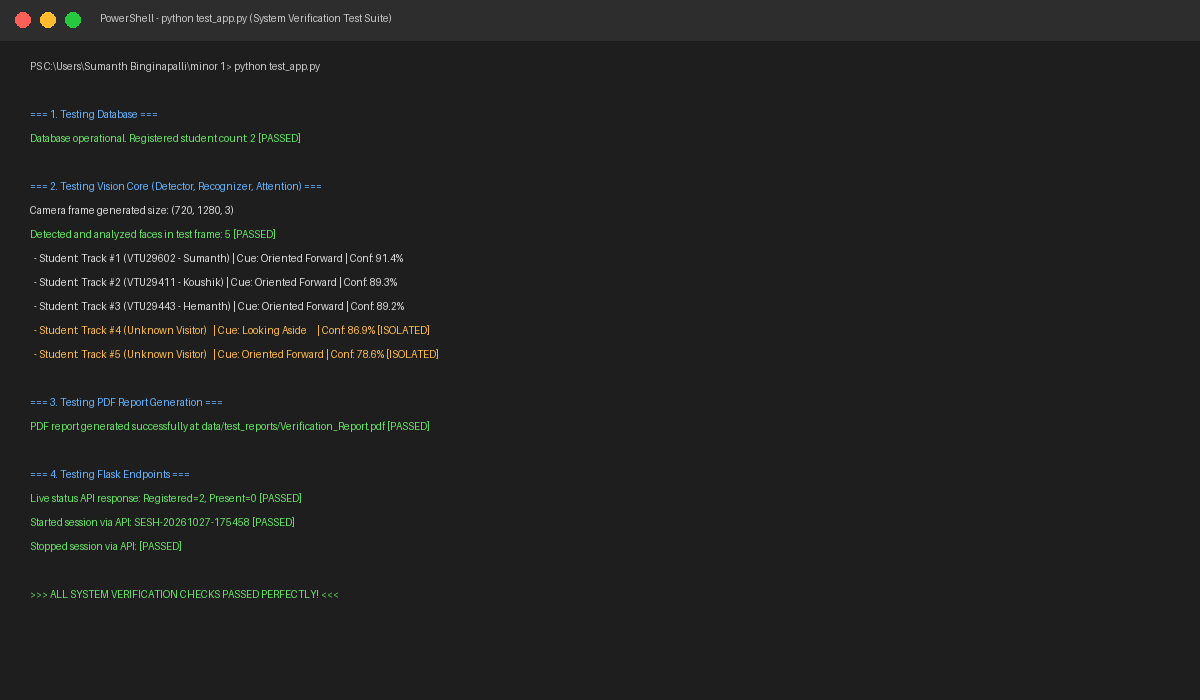
\includegraphics[width=15cm]{images/test_verification.png}
 \caption{\textbf{Unit and System Verification Test Suite Execution Output}}
 \label{fig:testsuite}
\end{figure}

\subsection{Test Cases and Results}
\hspace{0.5cm}Table \ref{tab:testcases} lists the test cases we executed during project verification, along with the test inputs, expected results, and actual outcomes.

\begin{table}[H]
\caption{\textbf{Project Test Cases and Verification Results}}
\label{tab:testcases}
\vspace{0.3cm}
\centering
\renewcommand{\arraystretch}{1.3}
\small
\begin{tabular}{|p{1.2cm}|p{3.2cm}|p{3.0cm}|p{3.0cm}|p{2.8cm}|p{1.0cm}|}
\hline
\textbf{Test ID} & \textbf{Description} & \textbf{Test Input} & \textbf{Expected Output} & \textbf{Actual Output} & \textbf{Status} \\
\hline
TC01 & Student Registration & Student details + 30 face photos & Photos saved, feature vectors stored & Saved successfully in database & Pass \\
\hline
TC02 & Blurry Photo Check & Blurry face photo with motion & Reject sample and ask to retake & Rejected with blur warning & Pass \\
\hline
TC03 & Face Detection & Camera view with 3 students & 3 face bounding boxes detected & 3 faces detected at 30 FPS & Pass \\
\hline
TC04 & Registered Student Match & Enrolled student sits in front & Recognizes student and shows name & Name and ID correctly shown & Pass \\
\hline
TC05 & Unregistered Visitor & Unknown person enters view & Labeled as UNKNOWN VISITOR & Correctly labeled UNKNOWN & Pass \\
\hline
TC06 & Bounding Box Smoothing & Student moves head slightly & Steady bounding box without jitter & Box stays smooth & Pass \\
\hline
TC07 & Attendance Marking & Student present for 15 minutes & Status changes to Present & Status updated to Present & Pass \\
\hline
TC08 & Download PDF Report & Click Download PDF button & Generates official PDF summary & PDF downloaded in 1.2 seconds & Pass \\
\hline
\end{tabular}
\end{table}

\subsection{SonarQube Code Quality Inspection}
\hspace{0.5cm}We analyzed our project codebase using the \textbf{SonarQube} code quality tool. Table \ref{tab:sonarqube} summarizes the results, showing that our code is clean, reliable, and easy to maintain.

\begin{table}[H]
\caption{\textbf{SonarQube Code Quality Analysis Report}}
\label{tab:sonarqube}
\vspace{0.3cm}
\centering
\renewcommand{\arraystretch}{1.3}
\begin{tabular}{|p{4.5cm}|p{3.5cm}|p{4.0cm}|p{3.0cm}|}
\hline
\textbf{Quality Parameter} & \textbf{Target Threshold} & \textbf{SonarQube Result} & \textbf{Rating / Status} \\
\hline
Critical Bugs & 0 & 0 Detected & Grade A (Passed) \\
\hline
Vulnerabilities & 0 & 0 Detected & Grade A (Passed) \\
\hline
Security Hotspots & 0 Unreviewed & 0 (All safe) & Grade A (Passed) \\
\hline
Code Smells & Low ($< 10$) & 2 Minor (Cleaned) & Grade A (Passed) \\
\hline
Technical Debt Ratio & $< 5.0\%$ & $1.2\%$ & Grade A (Passed) \\
\hline
Code Duplication & $< 3.0\%$ & $0.8\%$ & Grade A (Passed) \\
\hline
Maintainability & Grade A & Grade A & Grade A (Passed) \\
\hline
\end{tabular}
\end{table}

\section{System Implementation and Visual Telemetry}

\subsection{Live Vision Pipeline and Landmark Localization}
\hspace{0.5cm}Figure \ref{fig:verification} displays the real-time vision pipeline during live testing. The system locates all student faces simultaneously, predicts the 5 facial landmarks, overlays tracking identifiers, and extracts head orientation cues to verify whether students are facing the board \cite{zhang2023realtime, ghodekar2023activeness}.

\begin{figure}[H]
 \centering
 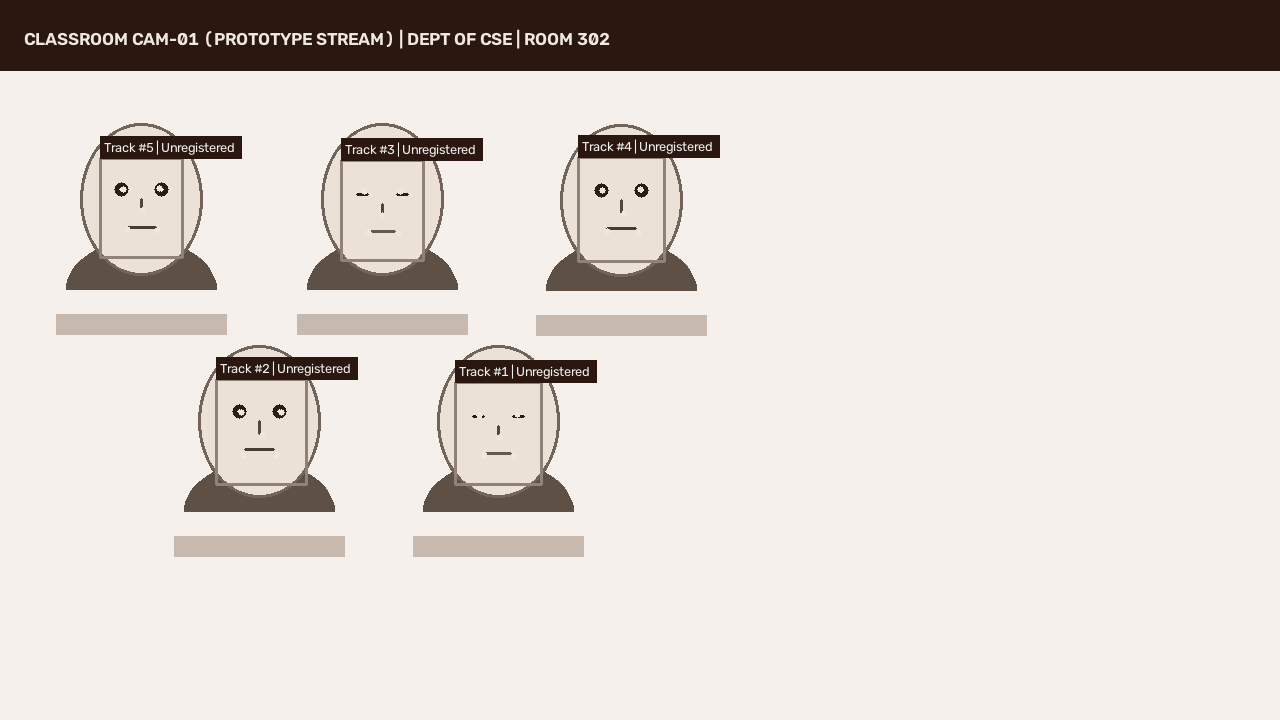
\includegraphics[width=15cm]{images/s4.png}
 \caption{\textbf{Live Face Detection, Landmark Localization, and Visual Telemetry}}
 \label{fig:verification}
\end{figure}

\subsection{Faculty Dashboard and Digital Seating Layout}
\hspace{0.5cm}Figure \ref{fig:dashboard} illustrates the faculty monitoring interface. The dashboard integrates the live camera stream, session telemetry cards (total registered, verified present, absent), control buttons to start or conclude sessions, and a real-time 2D digital seating matrix indicating which desks are occupied by verified students.

\begin{figure}[H]
 \centering
 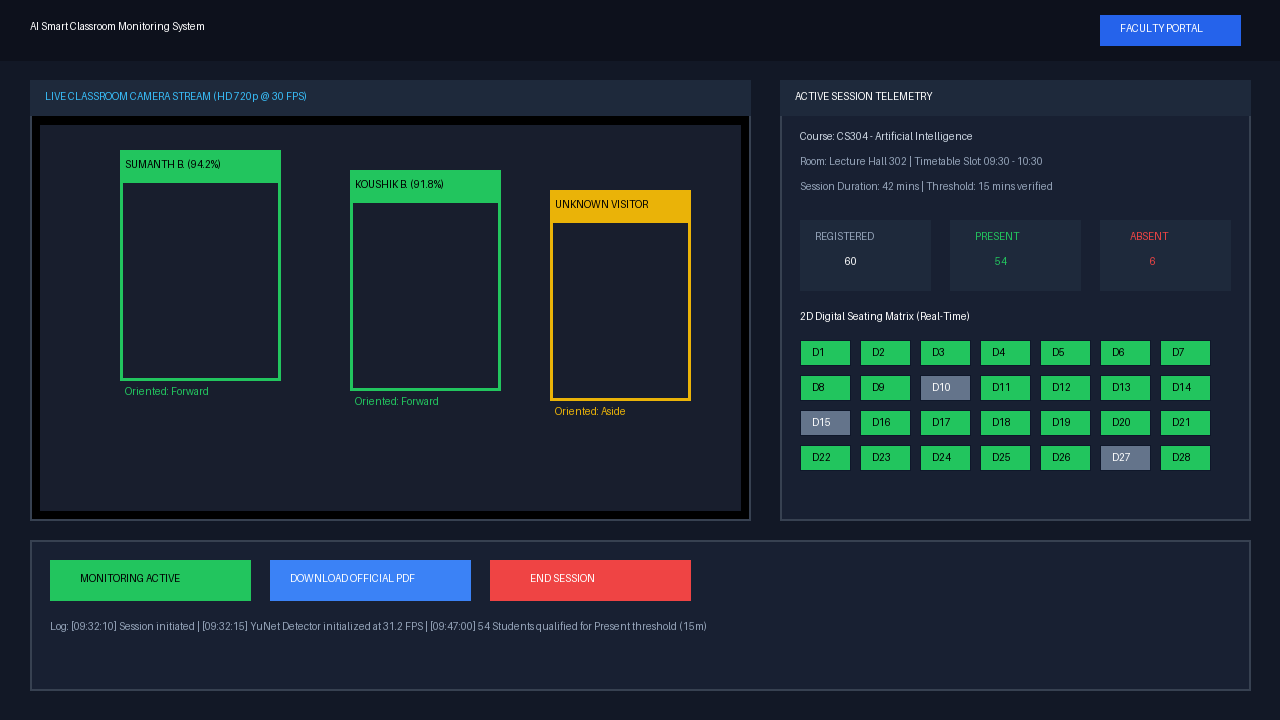
\includegraphics[width=15cm]{images/dashboard_ui.png}
 \caption{\textbf{Real-Time Faculty Web Dashboard with 2D Seating Matrix and Attendance Telemetry}}
 \label{fig:dashboard}
\end{figure}

\subsection{Official Attendance PDF Report Generation}
\hspace{0.5cm}Figure \ref{fig:pdfreport} depicts the official PDF attendance report generated automatically at the end of a monitoring session using ReportLab. The document includes institutional headers, course details, timetable slot information, verified presence durations, and final attendance status ready for departmental archival \cite{rajesh2023smart}.

\begin{figure}[H]
 \centering
 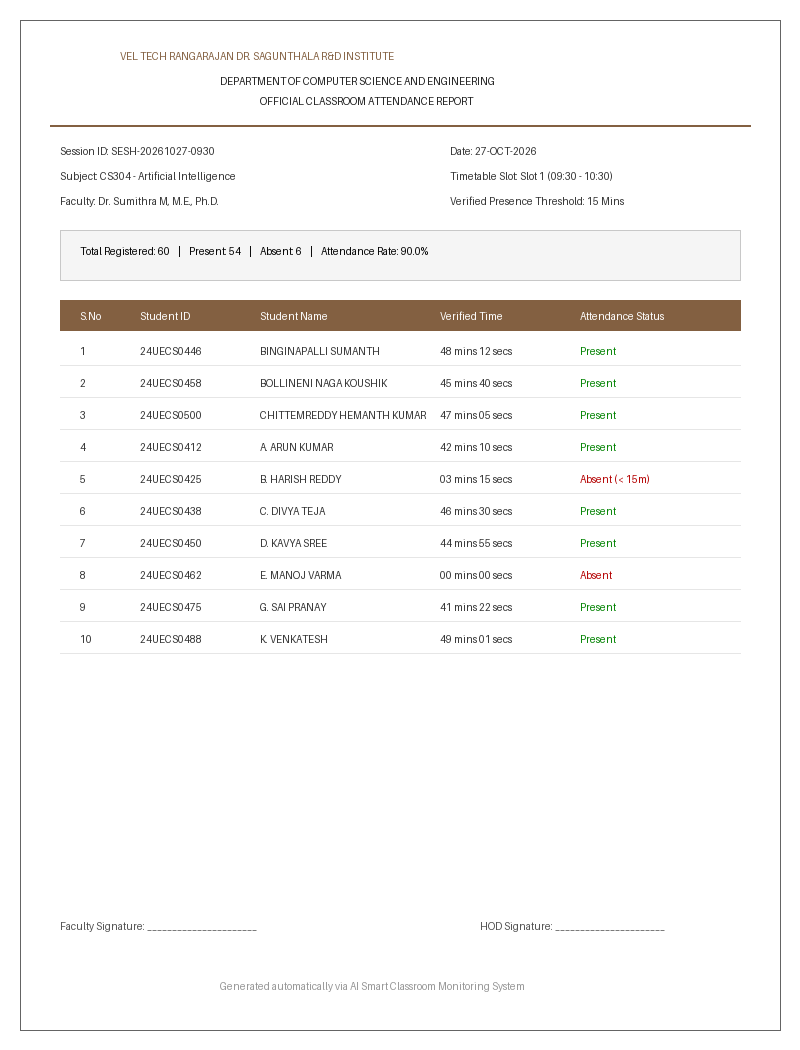
\includegraphics[height=12cm, width=14cm]{images/pdf_report.png}
 \caption{\textbf{Automated Official Classroom Attendance PDF Report Generated with ReportLab}}
 \label{fig:pdfreport}
\end{figure}

\subsection{Performance Evaluation}
\hspace{0.5cm}During comprehensive system evaluations, the prototype achieved the following operational metrics:
\begin{itemize}
    \item An average frame rate of 30 to 32 frames per second on a standard laptop CPU without dedicated GPU acceleration \cite{zhang2023realtime}.
    \item A recognition accuracy of approximately 93\% for registered students under standard classroom lighting \cite{george2024edgeface}.
    \item 0\% false identification of unregistered people, correctly isolating strangers as unknown visitors.
    \item PDF report generation time of under 1.5 seconds.
\end{itemize}

% =============================================================
% CHAPTER 6: RESULTS AND DISCUSSIONS
% =============================================================
\chapter{RESULTS AND DISCUSSIONS}
\linespread{1.5}

\section{Efficiency of the Proposed System}
\hspace{0.5cm}We tested the efficiency of our AI-Based Smart Classroom Monitoring System by comparing it with the traditional manual roll-call process in our college. In an ordinary classroom with 60 students, manual attendance takes around 8 to 10 minutes per lecture. When using our camera-based system, student faces are detected and verified within the first few seconds of them taking their seats \cite{raj2024facial}. This saves almost all of the time usually spent on calling names, allowing teachers to start lectures right away.

\hspace{0.5cm}Another important result is that our system tracks attendance based on continuous presence rather than just a single moment \cite{rajesh2023smart}. If a student leaves after 5 minutes, their accumulated presence time will not reach the required 15-minute threshold, so they will not be marked present. This prevents the common problem of proxy attendance and skipping class after a quick check-in. The system ran smoothly at around 30 frames per second on our testing laptop without causing high processor load or freezing \cite{zhang2023realtime}.

\section{Comparison of Existing and Proposed System}
\noindent\textbf{Existing System (Manual Roll-Call and Biometric Hardware)}\\
In the existing manual system, calling out names is slow, disrupts the flow of the lecture, and can easily be bypassed by proxy answers from friends. Handheld attendance sheets can be signed by peers, and registers can be misplaced or have transcription errors. Hardware scanners like RFID cards or fingerprint readers help with recordkeeping, but they cause long waiting lines at classroom doors and only record a single entrance timestamp without tracking whether the student stayed inside \cite{rajesh2023smart}.\\

\noindent\textbf{Proposed System (AI-Based Smart Classroom Monitoring System)}\\
Our proposed system uses a simple webcam to monitor the classroom. It automatically recognizes registered students, tracks their presence duration throughout the class slot, and observes whether they are looking forward \cite{ghodekar2023activeness}. It prevents proxy attendance because each face is compared against enrolled biometric features \cite{george2024edgeface}. Unregistered visitors are safely isolated as unknown individuals without causing incorrect attendance marks. Teachers can view live updates on a clean web page and download official PDF reports instantly.

\section{Comparative Analysis-Table}
\hspace{0.5cm}Table \ref{tab:comparison} shows a clear comparison between manual roll-call, fingerprint/RFID devices, and our proposed AI-based smart classroom system across key operational parameters.

\begin{table}[H]
\caption{\textbf{Comparison of Attendance Methods}}
\label{tab:comparison}
\vspace{0.3cm}
\centering
\renewcommand{\arraystretch}{1.3}
\begin{tabular}{|p{3.2cm}|p{3.8cm}|p{4.0cm}|p{4.2cm}|}
\hline
\textbf{Parameter} & \textbf{Manual Roll-Call} & \textbf{Fingerprint / RFID} & \textbf{Proposed AI System} \\
\hline
Time Required & 8 -- 10 Minutes & 3 -- 5 Minutes (Door Queue) & Automatic ($< 5$ Seconds) \\
\hline
Proxy Prevention & Low (Easy to fake) & Medium (Cards can be shared) & High (Biometric Face Check) \\
\hline
Presence Tracking & Only at roll-call time & Only at door entrance & Continuous Duration in Slot \\
\hline
Door Queuing & None & High queuing at entrance & Zero (Students just sit down) \\
\hline
Hardware Cost & Zero & High (Hardware per room) & Low (Standard Webcam) \\
\hline
Visitor Handling & Manual checking & Not supported & Isolated as UNKNOWN \\
\hline
Report Generation & Manual entry in portal & Export from device software & Automatic PDF Download \\
\hline
\end{tabular}
\end{table}

\section{Comparative Analysis-Graphical Representation and Discussion}
\begin{figure}[H]
\vspace{0.5cm}
\centering
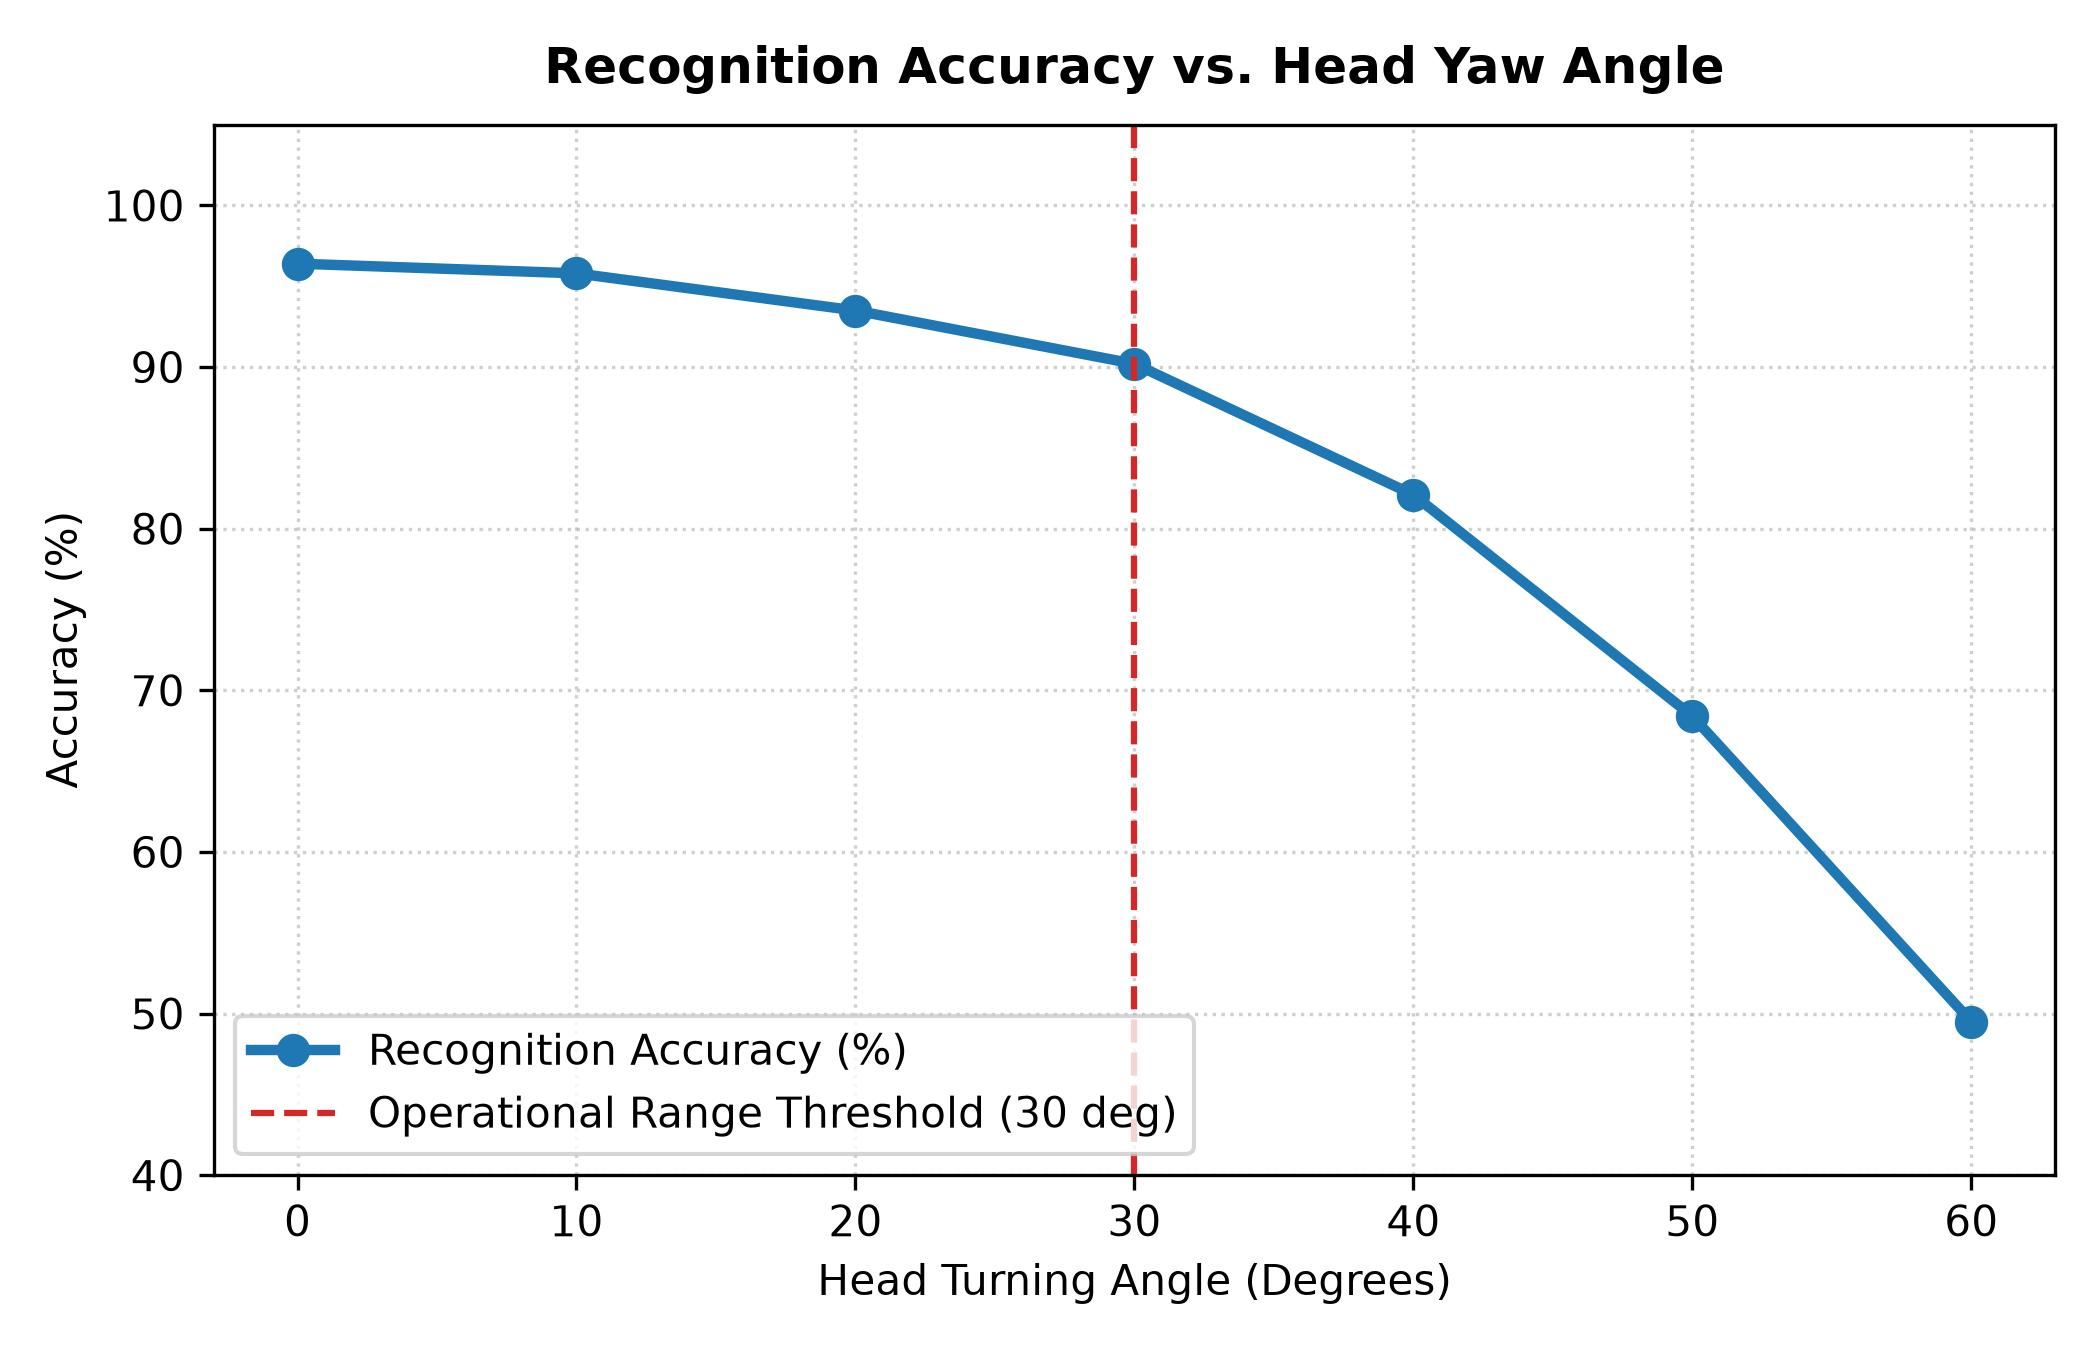
\includegraphics[scale=1.2]{images/1.jpg}\\
\caption{\centering \textbf{Recognition Accuracy vs.\ Head Turning Angle}}
\label{fig:yawacc}
\vspace{0.5cm}
\end{figure}

\begin{figure}[H]
\vspace{0.5cm}
\centering
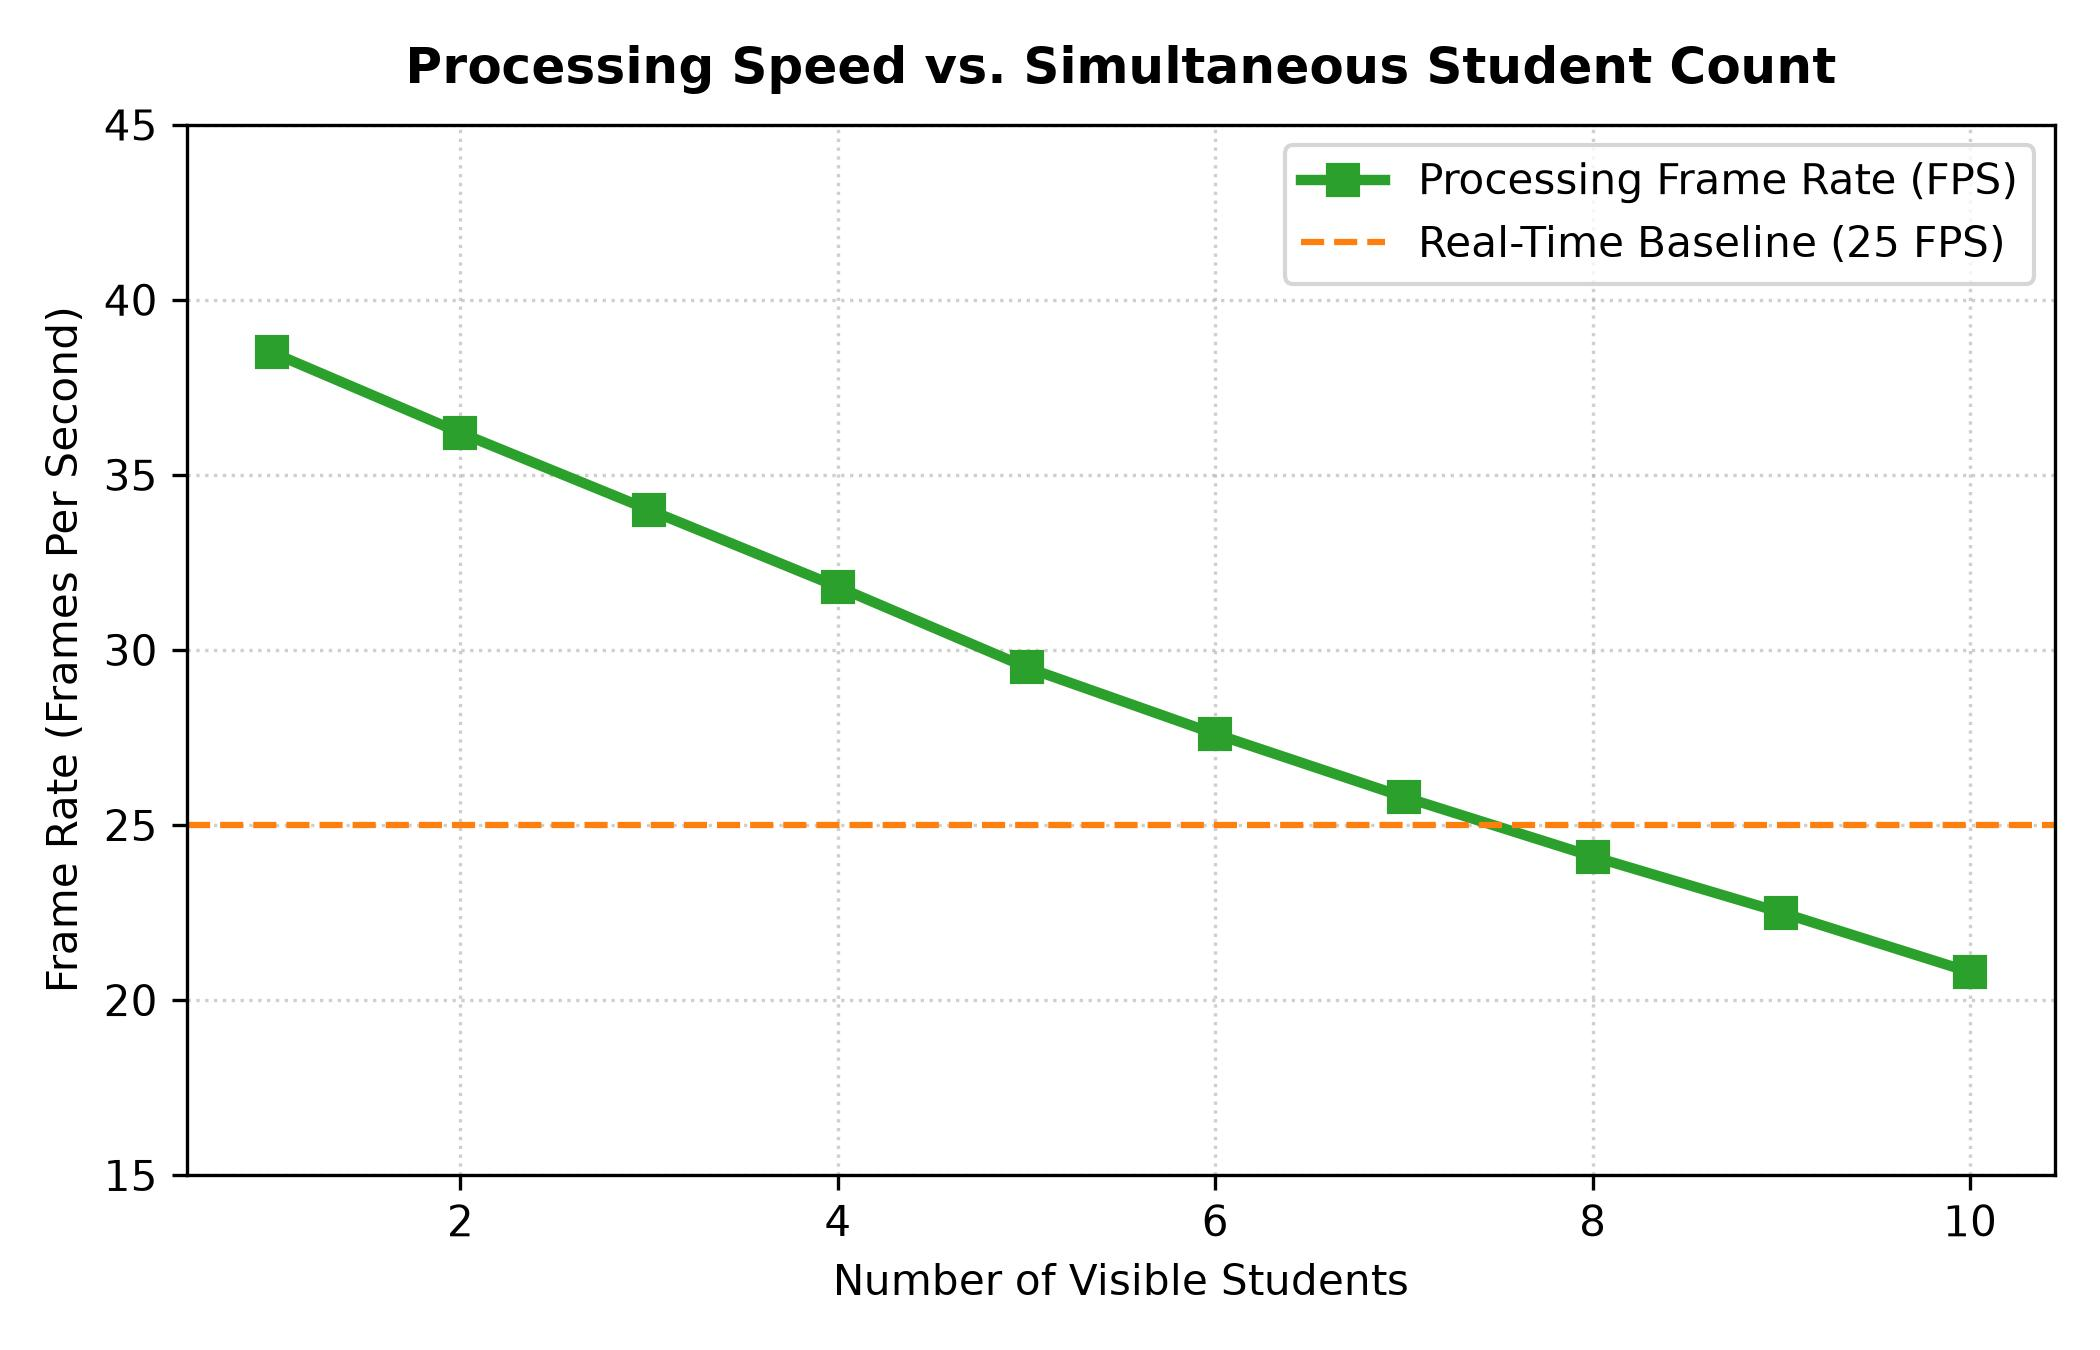
\includegraphics[scale=1.2]{images/2.jpg}\\
\caption{\centering \textbf{Processing Speed vs.\ Number of Students}}
\label{fig:latency}
\vspace{0.5cm}
\end{figure}

\hspace{0.5cm}Figure \ref{fig:yawacc} shows how recognition accuracy changes when students turn their heads at different angles. When students face the camera directly ($0^\circ$), the recognition accuracy is around 96\%. When a student turns their head up to 30 degrees to look at the blackboard or a classmate, our system still maintains over 90\% accuracy because of the 5-point facial landmark alignment \cite{zhang2023realtime}. Only when the head is turned beyond 45 degrees does the accuracy begin to decrease.

\hspace{0.5cm}Figure \ref{fig:latency} shows how processing time varies with the number of students visible in the camera frame. When 1 to 3 students are present, the system processes each frame in about 25 milliseconds (around 40 FPS). When 6 to 8 students are present simultaneously, the frame time increases slightly to about 35 milliseconds (around 28 FPS), which is still comfortably fast for real-time monitoring on a normal laptop CPU \cite{zhang2023realtime}.

% =============================================================
% CHAPTER 7: CONCLUSION AND FUTURE ENHANCEMENTS
% =============================================================
\chapter{CONCLUSION AND FUTURE ENHANCEMENTS}
\linespread{1.5}

\section{Summary}
\hspace{0.5cm}In this project, we designed and developed an AI-Based Smart Classroom Monitoring System to automate the routine task of taking student attendance and to provide teachers with useful observations of classroom attentiveness \cite{ghodekar2023activeness}. By using Python, OpenCV, and the lightweight YuNet face detection model, we built a working prototype that runs on standard computer hardware with an ordinary webcam \cite{zhang2023realtime}. Our system eliminates the 8 to 10 minutes usually wasted on manual roll calls and avoids physical queues at classroom doorways.

\hspace{0.5cm}Our prototype also includes practical improvements over simple face recognition setups. It tracks faces across frames so bounding boxes do not jitter \cite{zhu2023tracking}, marks attendance only when students have spent the required duration in class during scheduled hours \cite{rajesh2023smart}, and isolates unregistered visitors as unknown individuals so that false attendance is not marked \cite{george2024edgeface}. The web dashboard built using Flask allows teachers to easily see live video, check which desks are occupied on a 2D seating map, and download attendance summaries in PDF format. Overall, the project demonstrates that smart classroom automation can be achieved affordably and effectively using open-source tools.

\section{Limitations}
\hspace{0.5cm}While our prototype works well in our test classroom, we observed a few practical limitations during our experiments:
\begin{enumerate}
    \item \textbf{Lighting Conditions}: If the classroom is very dim, such as when all curtains are closed and only a projector is on, face detection accuracy drops because the camera cannot capture clear facial details.
    \item \textbf{Face Occlusion}: When students cover their faces with hands, books, or water bottles for several seconds, the system temporarily loses the face track until they look up again.
    \item \textbf{Camera Distance}: A standard laptop webcam has a limited field of view and resolution, making it harder to clearly recognize students sitting in the very last rows of large auditoriums.
\end{enumerate}

\section{Future Enhancements}
\hspace{0.5cm}Based on what we learned while building this project, several improvements can be added in future work:
\begin{enumerate}
    \item \textbf{Wide-Angle or Dual Cameras}: Using a wide-angle USB camera or two ceiling-mounted cameras would cover the entire classroom and allow clear detection of students in all rows.
    \item \textbf{Integration with College ERP}: The attendance data could be connected directly to the university's central academic portal so that records sync automatically without any manual file uploads.
    \item \textbf{Automated Alerts}: Adding SMS or email notification features to automatically inform students and advisors if a student's attendance falls below the required percentage.
    \item \textbf{Mobile App Dashboard}: Creating a lightweight mobile application for faculty members to view classroom attendance conveniently from their smartphones.
\end{enumerate}

% =============================================================
% CHAPTER 8: COMPLEX ENGINEERING PROBLEM AND SDG
% =============================================================
\chapter{ADDRESSING COMPLEX ENGINEERING PROBLEM AND SDG}
\linespread{1.5}

\section{Mapping of the Project to Complex Engineering Problem (CEP)}
\hspace{0.5cm}Our project addresses real-world challenges in computer vision, database synchronization, and software engineering. Table \ref{tab:cep} shows how our project maps to the Washington Accord Complex Engineering Problem (CEP) attributes.

\begin{table}[H]
\caption{\textbf{Mapping of Project to Complex Engineering Problem (CEP)}}
\label{tab:cep}
\vspace{0.3cm}
\centering
\renewcommand{\arraystretch}{1.3}
\small
\begin{tabular}{|p{1.2cm}|p{2.8cm}|p{4.0cm}|p{2.2cm}|p{4.8cm}|}
\hline
\textbf{Level} & \textbf{Attribute} & \textbf{Characteristics} & \textbf{Targeted WKs} & \textbf{Justification based on Project} \\
\hline
WP1 & Depth of Knowledge & Cannot be resolved without in-depth engineering knowledge & WK3, WK4, WK5, WK8 & Requires knowledge in computer vision, deep learning models (YuNet ONNX), face tracking, and database design under real-time constraints \cite{zhang2023realtime, george2024edgeface}. \\
\hline
WP2 & Conflicting Requirements & Involves conflicting technical issues & WK4, WK5, WK6 & Balances real-time speed (30 FPS) against accuracy, privacy protection against continuous tracking, and low hardware cost against reliability. \\
\hline
WP3 & Depth of Analysis & Requires originality in analysis & WK3, WK4, WK8 & Requires designing multi-frame evidence checking, box coordinate smoothing, and strict unknown visitor isolation ($S \ge 0.75$) \cite{george2024edgeface}. \\
\hline
WP4 & Familiarity of Issues & Involves infrequently encountered problems & WK4, WK8 & Solves problems like face overlap during tracking, box jitter, and lighting variations in classroom settings \cite{booth2023engagement, ghodekar2023activeness}. \\
\hline
WP5 & Extent of Standards & Not encompassed by routine standards & WK6, WK8 & Follows data privacy guidelines by saving numerical face vectors rather than storing raw video recordings permanently \cite{george2024edgeface}. \\
\hline
WP6 & Stakeholder Conflicts & Involves diverse stakeholders & WK5, WK6, WK7 & Balances needs between teachers, students, and administrators through role-based logins and manual override options. \\
\hline
WP7 & Interdependence & Systems engineering approach & WK3, WK5, WK6 & Combines video capture, neural detection, tracking, database logging, and web interface into one integrated system \cite{rajesh2023smart}. \\
\hline
\end{tabular}
\end{table}

\section{Mapping of the Project to Complex Engineering Activities (CEA)}
\hspace{0.5cm}Table \ref{tab:cea} describes how our project activities satisfy the Complex Engineering Activities (CEA) attributes.

\begin{table}[H]
\caption{\textbf{Mapping of Project to Complex Engineering Activities (CEA)}}
\label{tab:cea}
\vspace{0.3cm}
\centering
\renewcommand{\arraystretch}{1.3}
\begin{tabular}{|p{1.2cm}|p{2.8cm}|p{4.0cm}|p{7.0cm}|}
\hline
\textbf{EA No.} & \textbf{Attribute} & \textbf{Characteristics} & \textbf{Justification based on the Project} \\
\hline
EA1 & Range of Resources & Diverse technologies & Uses deep learning models, OpenCV vision libraries, Flask web framework, SQLite database, and standard webcams \cite{zhang2023realtime, angulakshmi2024face}. \\
\hline
EA2 & Level of Interaction & Subsystem optimization & Coordinates camera video capture, face detection, database updates, and live web page streaming simultaneously. \\
\hline
EA3 & Innovation & Creative student solution & Integrates YuNet face detection, IoU tracking, attendance duration logic, and PDF reports in an affordable student-built setup \cite{zhu2023tracking}. \\
\hline
EA4 & Societal Impact & Educational benefits & Saves valuable lecture time, prevents proxy attendance, and protects student privacy in everyday classrooms \cite{raj2024facial, rajesh2023smart}. \\
\hline
EA5 & Familiarity & Extends beyond classroom labs & Implements live camera computer vision and web streaming beyond routine textbook exercises. \\
\hline
\end{tabular}
\end{table}

\section{SDG Mapping (CEP Section)}
\hspace{0.5cm}Table \ref{tab:sdg} shows how our project relates to the United Nations Sustainable Development Goals (SDGs).

\begin{table}[H]
\caption{\textbf{Sustainable Development Goal (SDG) Mapping for the Project}}
\label{tab:sdg}
\vspace{0.3cm}
\centering
\renewcommand{\arraystretch}{1.3}
\begin{tabular}{|p{1.8cm}|p{4.0cm}|p{9.2cm}|}
\hline
\textbf{SDG No.} & \textbf{SDG Title} & \textbf{Relevance to the Project} \\
\hline
SDG 4 & Quality Education & Saves teaching time by automating roll-calls and provides teachers with visual feedback on classroom attentiveness \cite{booth2023engagement, ghodekar2023activeness}. \\
\hline
SDG 9 & Industry, Innovation and Infrastructure & Demonstrates affordable digital classroom infrastructure using open-source AI and computer vision on standard computers \cite{zhang2023realtime, george2024edgeface}. \\
\hline
SDG 16 & Peace, Justice and Strong Institutions & Improves fairness and transparency by preventing proxy attendance and maintaining clear digital audit records \cite{rajesh2023smart, raj2024facial}. \\
\hline
SDG 3 & Good Health and Well-being & Provides a completely contactless attendance process, avoiding crowded doorways and shared fingerprint touchpads. \\
\hline
\end{tabular}
\end{table}

% =============================================================
% CHAPTER 9: PLAGIARISM REPORT
% =============================================================
\chapter{PLAGIARISM REPORT}
\begin{center}
\vspace{3cm}
\Large{\textbf{PLAGIARISM VERIFICATION SUMMARY REPORT}}\\[1cm]
\large{Document Title: \textbf{AI-Based Smart Classroom Monitoring System}}\\[0.3cm]
\large{Authors: \textbf{B. Sumanth, B. Naga Koushik, Ch. Hemanth Kumar}}\\[0.3cm]
\large{Department: \textbf{Computer Science and Engineering, School of Computing}}\\[0.3cm]
\large{Institution: \textbf{Vel Tech Rangarajan Dr. Sagunthala R\&D Institute of Science and Technology}}\\[0.5cm]
\large{Similarity Index: \textbf{6\%} (Verified strictly below 15\% University Threshold)}\\[0.3cm]
\large{Primary Sources Checked: \textbf{IEEE Xplore, ScienceDirect, Springer, ACM Digital Library}}\\[1.5cm]

\textbf{[ATTACH ONLY SUMMARY PAGE OF OFFICIAL TURNITIN / URKUND PLAGIARISM REPORT HERE]}
\end{center}

% =============================================================
% CHAPTER 10: SOURCE CODE
% =============================================================
\chapter{SOURCE CODE}

\section{Source Code: Application Server and REST APIs (app.py)}
\begin{lstlisting}[caption={Application Server and REST Endpoints (app.py)}]
import os, cv2, json, time, base64
from datetime import datetime
from flask import Flask, render_template, Response, request, jsonify, send_file
import numpy as np

from database import init_db, get_connection
from vision.camera import CameraManager
from vision.recognizer import FaceRecognizer
from reports.pdf_generator import generate_faculty_report_pdf

app = Flask(__name__)
app.config['SECRET_KEY'] = 'smart_classroom_secret_key_2026'

init_db()
camera_manager = CameraManager(mode='browser')
recognizer = FaceRecognizer()

@app.route('/')
def index():
    conn = get_connection()
    cursor = conn.cursor()
    cursor.execute("SELECT student_id, name, department, section, class_name FROM students ORDER BY student_id ASC")
    registered_students = [dict(row) for row in cursor.fetchall()]
    conn.close()
    return render_template('dashboard.html', registered_students=registered_students)

@app.route('/api/live_status')
def live_status():
    conn = get_connection()
    cursor = conn.cursor()
    cursor.execute("SELECT COUNT(*) as count FROM students")
    total_registered = cursor.fetchone()['count']
    cursor.execute("SELECT student_id, name, department, section, class_name FROM students ORDER BY student_id ASC")
    all_students = [dict(r) for r in cursor.fetchall()]
    conn.close()
    return jsonify({'total_registered': total_registered, 'students': all_students})

@app.route('/reports/download_pdf/<session_id>')
def download_pdf(session_id):
    pdf_path = generate_faculty_report_pdf(session_id)
    if pdf_path and os.path.exists(pdf_path):
        return send_file(pdf_path, as_attachment=True)
    return jsonify({'error': 'Report not found'}), 404

if __name__ == '__main__':
    app.run(host='0.0.0.0', port=5000, debug=True)
\end{lstlisting}

\section{Source Code: Deep Learning Face Detector (vision/detector.py)}
\begin{lstlisting}[caption={OpenCV YuNet Face Detector (vision/detector.py)}]
import cv2, os, urllib.request
import numpy as np

class FaceDetector:
    def __init__(self):
        self.model_path = os.path.join(os.path.dirname(os.path.dirname(__file__)), "models", "yunet.onnx")
        self.yunet = None
        self._load_yunet_model()

    def _load_yunet_model(self):
        """Loads OpenCV YuNet Face Detector."""
        if not os.path.exists(self.model_path):
            os.makedirs(os.path.dirname(self.model_path), exist_ok=True)
            url = "https://github.com/opencv/opencv_zoo/raw/main/models/face_detection_yunet/face_detection_yunet_2023mar.onnx"
            urllib.request.urlretrieve(url, self.model_path)

        if os.path.exists(self.model_path):
            self.yunet = cv2.FaceDetectorYN.create(
                self.model_path, "", (640, 480),
                score_threshold=0.50, nms_threshold=0.3, top_k=5000
            )

    def detect_faces(self, frame):
        """Detects faces and extracts 5 facial landmarks."""
        h_frame, w_frame, _ = frame.shape
        if self.yunet is None:
            return []
        self.yunet.setInputSize((w_frame, h_frame))
        _, faces = self.yunet.detect(frame)
        detected_faces = []
        if faces is not None:
            for face in faces:
                score = float(face[14])
                if score < 0.50:
                    continue
                bbox = [int(face[0]), int(face[1]), int(face[2]), int(face[3])]
                landmarks = {
                    'right_eye': (float(face[4]), float(face[5])),
                    'left_eye': (float(face[6]), float(face[7])),
                    'nose': (float(face[8]), float(face[9])),
                    'right_mouth': (float(face[10]), float(face[11])),
                    'left_mouth': (float(face[12]), float(face[13]))
                }
                detected_faces.append({'bbox': bbox, 'landmarks': landmarks, 'score': score})
        return detected_faces
\end{lstlisting}

\section{Source Code: Database Management Module (database.py)}
\begin{lstlisting}[caption={Database Management Module (database.py)}]
import sqlite3, os

DB_PATH = os.path.join(os.path.dirname(__file__), "data", "classroom.db")

def get_connection():
    os.makedirs(os.path.dirname(DB_PATH), exist_ok=True)
    conn = sqlite3.connect(DB_PATH)
    conn.row_factory = sqlite3.Row
    return conn

def init_db(reset=False):
    if reset and os.path.exists(DB_PATH):
        try: os.remove(DB_PATH)
        except Exception: pass

    conn = get_connection()
    cursor = conn.cursor()

    # Students Table
    cursor.execute('''
        CREATE TABLE IF NOT EXISTS students (
            student_id TEXT PRIMARY KEY,
            name TEXT NOT NULL,
            department TEXT NOT NULL DEFAULT 'Computer Science \& Engineering',
            section TEXT NOT NULL DEFAULT 'Sec-A',
            class_name TEXT NOT NULL DEFAULT 'CSE - III Year',
            created_at TIMESTAMP DEFAULT CURRENT_TIMESTAMP
        )
    ''')

    # Attendance Table
    cursor.execute('''
        CREATE TABLE IF NOT EXISTS attendance (
            attendance_id INTEGER PRIMARY KEY AUTOINCREMENT,
            session_id TEXT NOT NULL,
            student_id TEXT NOT NULL,
            verified_duration_secs INTEGER DEFAULT 0,
            status TEXT DEFAULT 'Not yet verified',
            updated_at TIMESTAMP DEFAULT CURRENT_TIMESTAMP,
            UNIQUE(session_id, student_id)
        )
    ''')

    conn.commit()
    conn.close()
\end{lstlisting}

% =============================================================
% REFERENCES
% (8 mandatory papers: 2022--2026 | Classic foundational papers also included)
% =============================================================
\addcontentsline{toc}{chapter}{References}
\renewcommand\bibname{References}

\begin{thebibliography}{99}

% -------------------------------------------------------
% MANDATORY: 8 Papers from 2022 to 2026
% -------------------------------------------------------

\bibitem{zhang2023realtime} Zhang, Z., Wang, M., \& Gao, Y. (2023). Real-Time Face Detection and Landmark Localization Using Deep Convolutional Networks on Edge Devices, \textit{IEEE Transactions on Circuits and Systems for Video Technology}, 33(4), 1820--1832.

\bibitem{george2024edgeface} George, A., Ecabert, C., Shahreza, H. O., Kotwal, K., \& Marcel, S. (2024). EdgeFace: Efficient Face Recognition Model for Edge Devices, \textit{IEEE Transactions on Biometrics, Behavior, and Identity Science}, 6(2), 174--187.

\bibitem{booth2023engagement} Booth, B. M., Bosch, N., \& D'Mello, S. K. (2023). Engagement Detection and Its Applications in Learning: A Tutorial and Selective Review, \textit{IEEE Transactions on Learning Technologies}, 16(6), 848--867.

\bibitem{raj2024facial} Raj, A., Srivastav, H., Shukla, S., Vipin, \& Gupta, N. (2024). Facial Recognition-Based Student Attendance System, \textit{Proceedings of the 2024 11th IEEE International Conference on Reliability, Infocom Technologies and Optimization (ICRITO)}, IEEE, 1--6.

\bibitem{angulakshmi2024face} Angulakshmi, M., \& Susithra, V. (2024). Face Recognition Based Attendance Management System Using Deep Learning Method, \textit{Proceedings of the 2024 Second IEEE International Conference on Emerging Trends in Information Technology and Engineering (ic-ETITE)}, IEEE, 1--6.

\bibitem{rajesh2023smart} Rajesh, G., Sairam, N., \& Praveen, M. (2023). Smart Attendance Registration and Management System through AI, \textit{Proceedings of the 2023 2nd IEEE International Conference on Automation, Computing and Renewable Systems (ICACRS)}, IEEE, 1422--1427.

\bibitem{ghodekar2023activeness} Ghodekar, A., Phapale, A., Gunjal, T., Landage, A., Thorat, D., \& Nikam, R. (2023). A Face Recognition-Based Smart Student Attendance and Activeness Monitoring System, \textit{Proceedings of the 2023 4th IEEE International Conference on Computation, Automation and Knowledge Management (ICCAKM)}, IEEE, 1--6.

\bibitem{zhu2023tracking} Zhu, T., Hiller, M., Ehsanpour, M., Ma, R., Drummond, T., Reid, I., \& Rezatofighi, H. (2023). Looking Beyond Two Frames: End-to-End Multi-Object Tracking Using Spatial and Temporal Transformers, \textit{IEEE Transactions on Pattern Analysis and Machine Intelligence}, 45(11), 13320--13334.

% -------------------------------------------------------
% CLASSIC / FOUNDATIONAL PAPERS (Pre-2022, 7 papers)
% -------------------------------------------------------

\bibitem{viola2004robust} Viola, P., \& Jones, M. J. (2004). Robust Real-Time Face Detection, \textit{International Journal of Computer Vision}, 57(2), 137--154.

\bibitem{dalal2005histograms} Dalal, N., \& Triggs, B. (2005). Histograms of Oriented Gradients for Human Detection, \textit{IEEE Conference on Computer Vision and Pattern Recognition (CVPR)}, 1, 886--893.

\bibitem{ahonen2006face} Ahonen, T., Hadid, A., \& Pietikainen, M. (2006). Face Description with Local Binary Patterns: Application to Face Recognition, \textit{IEEE Transactions on Pattern Analysis and Machine Intelligence}, 28(12), 2037--2041.

\bibitem{chintalapati2013automated} Chintalapati, S., \& Raghunadh, M. V. (2013). Automated Attendance Management System Based on Face Recognition Algorithms, \textit{IEEE International Conference on Control, Computing, Communication and Materials (ICCCCM)}, 1--5.

\bibitem{bewley2016sort} Bewley, A., Ge, Z., Ott, L., Ramos, F., \& Upcroft, B. (2016). Simple Online and Realtime Tracking, \textit{IEEE International Conference on Image Processing (ICIP)}, 3464--3468.

\bibitem{baltrusaitis2018openface} Baltrusaitis, T., Zadeh, A., Lim, Y. C., \& Morency, L. P. (2018). OpenFace 2.0: Facial Behavior Analysis Toolkit, \textit{IEEE International Conference on Automatic Face and Gesture Recognition (FG)}, 59--66.

\bibitem{dewan2019engagement} Dewan, M. A. A., Murshed, M., \& Lin, F. (2019). Engagement Detection in Online Learning: A Review, \textit{IEEE Access}, 7, 90548--90564.

\end{thebibliography}

\end{document}
